\documentclass[12pt,a4paper]{report}
\usepackage[utf8]{inputenc}
\usepackage[T1]{fontenc}
\usepackage[french]{babel}
\usepackage{geometry}
\geometry{margin=2.5cm, top=2.5cm, bottom=3.2cm, footskip=1.5cm, headheight=15pt}
\widowpenalty10000
\clubpenalty10000
\usepackage{times} % Times New Roman
\usepackage{hyperref}
\usepackage{xcolor}
\usepackage{graphicx}
\usepackage{tabularx}
\usepackage{booktabs}
\usepackage{titlesec}
\usepackage{fancyhdr}
\usepackage{float}
\usepackage{caption}
\usepackage{subcaption}
\usepackage{listings}
\usepackage{amsmath}
\usepackage{amssymb}
\usepackage{enumitem}
\usepackage{setspace}
\usepackage{longtable}
\usepackage{array}

\usepackage{tikz}
\usetikzlibrary{positioning, arrows.meta, shapes.geometric, calc, shadows}

% Définition des couleurs exactes du modèle
\definecolor{emsiblue}{RGB}{68, 114, 196}
\definecolor{emsigreen}{RGB}{112, 173, 71} % Vert à gauche
\definecolor{emsimaroon}{RGB}{146, 38, 42} % Grenat en bas
\definecolor{lightgray}{RGB}{245, 245, 245}

% Configuration des liens
\hypersetup{
    colorlinks=true,
    linkcolor=black,
    citecolor=black,
    filecolor=magenta,      
    urlcolor=emsiblue,
    pdftitle={Rapport PFA - ManageraHub},
}

% Style des chapitres et sections
\titleformat{\chapter}[display]
  {\normalfont\huge\bfseries\color{emsiblue}}
  {\chaptertitlename\ \thechapter}{10pt}{\Huge}

\titleformat{\section}
  {\normalfont\Large\bfseries\color{emsiblue}}
  {\thesection}{1em}{}

\titleformat{\subsection}
  {\normalfont\large\bfseries\color{emsiblue}}
  {\thesubsection}{1em}{}

% En-tête et pied de page
\pagestyle{fancy}
\fancyhf{}
\fancyhead[L]{\small \itshape Rapport de Projet de Fin d'Année - 3\textsuperscript{ème} IIR}
\fancyhead[R]{\small \itshape ManageraHub}
\fancyfoot[C]{\color{emsiblue} \large\bfseries \thepage}
\renewcommand{\headrulewidth}{0.4pt}

% Redéfinition du style plain (utilisé par défaut sur les pages de début de chapitre) pour avoir le même footer
\fancypagestyle{plain}{
    \fancyhf{}
    \fancyfoot[C]{\color{emsiblue} \large\bfseries \thepage}
    \renewcommand{\headrulewidth}{0pt}
}

\onehalfspacing

% Commande personnalisée pour les placeholders de captures d'écran
\newcommand{\screenshotplaceholder}[2][8cm]{
    \begin{figure}[H]
        \centering
        \begin{tikzpicture}
            % Simulated Browser window frame
            \draw[draw=emsiblue!60, fill=lightgray!10, thick, rounded corners=6pt] (0,0) rectangle (\textwidth,#1);
            % Title bar
            \draw[draw=emsiblue!60, fill=emsiblue!15, thick, rounded corners=6pt] (0,#1) -- (0,#1-0.8cm) -- (\textwidth,#1-0.8cm) -- (\textwidth,#1) -- cycle;
            % Minimize, Maximize, Close buttons
            \fill[red!80] (0.4cm, #1-0.4cm) circle (0.12cm);
            \fill[orange!80] (0.8cm, #1-0.4cm) circle (0.12cm);
            \fill[green!80] (1.2cm, #1-0.4cm) circle (0.12cm);
            % URL bar
            \draw[draw=gray!30, fill=white, rounded corners=3pt] (1.8cm, #1-0.6cm) rectangle (\textwidth-0.4cm, #1-0.2cm);
            \node[anchor=west, font=\ttfamily\scriptsize\color{gray}] at (2.0cm, #1-0.4cm) {https://www.managerahub.ma/};
            
            % Mock UI elements inside the window
            \node[emsiblue!80, font=\Large\bfseries] at (\textwidth/2, #1/2 + 0.6cm) {ManageraHub};
            \node[gray!90, font=\large\bfseries, align=center] at (\textwidth/2, #1/2) {#2};
            \node[gray!50, align=center, font=\scriptsize\itshape] at (\textwidth/2, #1/2 - 0.7cm) {Interface de l'application - Rendu Web d'illustration};
        \end{tikzpicture}
        \caption{#2}
    \end{figure}
}

% Configuration des listings de code
\lstset{
    backgroundcolor=\color{lightgray},
    basicstyle=\ttfamily\small,
    breakatwhitespace=false,
    breaklines=true,
    captionpos=b,
    commentstyle=\color{emsigreen},
    keywordstyle=\color{emsimaroon}\bfseries,
    stringstyle=\color{emsiblue},
    frame=single,
    keepspaces=true,
    numbers=left,
    numberstyle=\tiny\color{gray},
    showspaces=false,
    showstringspaces=false,
    showtabs=false,
    tabsize=2,
    language=Python
}

\begin{document}

% --- Pages préliminaires (chiffres romains) ---
\pagenumbering{roman}

\begin{titlepage}
    \begin{tikzpicture}[remember picture, overlay]
        \fill[emsigreen] ($(current page.north west) + (1.5cm,-2cm)$) rectangle ($(current page.south west) + (1.8cm,2cm)$);
        \fill[emsimaroon] ($(current page.south west) + (2cm,2.5cm)$) rectangle ($(current page.south east) + (-2cm,2.7cm)$);
        \fill[emsimaroon] ($(current page.south east) + (-1.8cm,2.5cm)$) rectangle ($(current page.south east) + (-1.4cm,2.9cm)$);
    \end{tikzpicture}

    \centering
    \begin{minipage}{0.5\textwidth}
        
\includegraphics[width=\textwidth,height=1.8cm,keepaspectratio]{logo_0.png}
    \end{minipage}%
    \hfill
    \begin{minipage}{0.4\textwidth}
        \hfill
\includegraphics[width=\textwidth,height=1.8cm,keepaspectratio]{logo_1.png}
    \end{minipage}
    
    \vspace{1.5cm}
    
    {\Large \textbf{Rapport de Projet de Fin d'Année (PFA)}} \\
    \vspace{0.4cm}
    {\large \textbf{Filière : Ingénierie Informatique et Réseaux (IIR)}} \\
    \vspace{0.4cm}
    {\large \textbf{Niveau : 3\textsuperscript{ème} année}} \\
    
    \vfill
    
    {\Huge \textbf{\color{emsiblue} ManageraHub}} \\
    \vspace{0.6cm}
    {\Large \textbf{\color{emsiblue} Application Web de Gestion des Candidatures d'Emploi}} \\
    
    \vfill
    
    \vspace{1.5cm}
    
    \begin{minipage}{0.48\textwidth}
        \begin{flushleft} \large
            \textbf{Réalisé par :}\\
            \vspace{0.2cm}
            Tchich Adam \\
            Rajiallah Aya
        \end{flushleft}
    \end{minipage}
    \hfill
    \begin{minipage}{0.48\textwidth}
        \begin{flushright} \large
            \textbf{Encadré par :} \\
            \vspace{0.2cm}
            Pr. Mme Nasr Nora
        \end{flushright}
    \end{minipage}
    
    \vfill
    
    {\large \textbf{ANNÉE UNIVERSITAIRE : 2025-2026}}
    \vspace{1cm}
\end{titlepage}

\chapter*{Dédicaces}
\addcontentsline{toc}{chapter}{Dédicaces}
\markboth{Dédicaces}{Dédicaces}

\vspace*{2cm}

\begin{center}
    \large
    \emph{À nos chers parents, \\
    Qui ont œuvré toute leur vie pour notre éducation, \\
    Pour leur amour inconditionnel, leurs sacrifices constants, \\
    Et leur soutien indéfectible à chaque étape de notre vie. \\
    Aucun mot ne saurait exprimer notre profonde gratitude.}
    
    \vspace{1.5cm}
    
    \emph{À nos familles et proches, \\
    Pour leur présence chaleureuse et leurs encouragements quotidiens.}
    
    \vspace{1.5cm}
    
    \emph{À nos enseignants de l'École Marocaine des Sciences de l'Ingénieur (EMSI), \\
    Qui nous ont transmis le savoir avec passion et rigueur, \\
    Et qui ont forgé notre esprit d'ingénieur.}
    
    \vspace{1.5cm}
    
    \emph{À tous ceux qui aiment la science et le progrès informatique, \\
    Nous dédions ce modeste travail.}
\end{center}
\newpage

\chapter*{Remerciements}
\addcontentsline{toc}{chapter}{Remerciements}
\markboth{Remerciements}{Remerciements}

Avant tout développement sur ce projet, nous tenons à exprimer notre profonde gratitude envers toutes les personnes qui ont contribué, de près ou de loin, à l'aboutissement de ce projet de fin d'année et à la rédaction de ce rapport.

\vspace{0.5cm}

Nous tenons à remercier en tout premier lieu notre encadrante pédagogique, \textbf{Pr. Mme Nasr Nora}, pour avoir accepté d'encadrer ce projet. Ses précieux conseils, ses directives méthodologiques pertinentes, sa rigueur scientifique et sa grande disponibilité tout au long du projet ont été des éléments indispensables pour notre progression et la réussite de nos tâches.

\vspace{0.5cm}

Nos remerciements s'adressent également à l'ensemble des professeurs et au personnel administratif de l'\textbf{École Marocaine des Sciences de l'Ingénieur (EMSI) de Rabat} pour la qualité de la formation dispensée, leur dévouement constant et les opportunités professionnelles qu'ils offrent aux étudiants ingénieurs.

\vspace{0.5cm}

Enfin, nous remercions nos familles et nos amis pour leur patience infinie, leur soutien moral indéfectible et leur confiance continue durant toute cette année universitaire.
\newpage

\chapter*{Résumé}
\addcontentsline{toc}{chapter}{Résumé}
\markboth{Résumé}{Résumé}

Le projet \textbf{ManageraHub} est une plateforme web moderne conçue pour répondre de manière innovante et sécurisée aux besoins croissants de recrutement et de réseautage professionnel sur le marché de l'emploi au Maroc. Face à la prolifération croissante de fausses offres d'emploi et d'usurpations d'identité d'entreprises sur les canaux de communication informels, ManageraHub introduit un mécanisme d'approbation et de vérification administrative obligatoire pour toutes les entités de recrutement. Ce processus de validation rigoureux s'appuie sur la soumission de documents officiels légaux, tels que l'Identifiant Commun de l'Entreprise (ICE) et le Registre du Commerce (RC), permettant d'instaurer une confiance totale entre les candidats et les employeurs.

Développée avec le framework de haut niveau \textbf{Django} et structurée selon le paradigme Model-View-Template (MVT), la plateforme offre une expérience utilisateur riche combinant recrutement classique et réseautage social professionnel. Les candidats bénéficient d'un profil interactif complet incluant la gestion multicritère de leurs compétences, de leurs expériences professionnelles et de certifications multiples. Les recruteurs disposent d'un tableau de bord de pilotage ergonomique facilitant la publication d'offres et le traitement collaboratif des statuts de postulation (en attente, entretien planifié, acceptée, refusée). De plus, le fil d'actualités sociales intégré permet la publication de posts, le partage d'expériences professionnelles et des micro-interactions de type "likes" et commentaires, tout en offrant la possibilité de taguer des profils professionnels et des entreprises vérifiées.

Ce rapport retrace l'ensemble des étapes clés du projet en s'appuyant sur le processus unifié \textbf{2TUP} (2 Track Unified Process). Il expose l'étude de l'existant, la planification par les diagrammes de Gantt et PERT, la conception UML complète ainsi que les choix technologiques et les détails d'implémentation frontend et backend sécurisés.

\vspace{0.5cm}
\noindent \textbf{Mots clés :} Django, Recrutement, Réseautage Social, UML, Vérification ICE, Python, Web Sécurisé, 2TUP.

\newpage

\chapter*{Abstract}
\addcontentsline{toc}{chapter}{Abstract}
\markboth{Abstract}{Abstract}

The \textbf{ManageraHub} project is a modern web platform designed to provide an innovative and secure solution to the growing challenges of recruitment and professional networking in the Moroccan job market. Addressing the proliferation of fraudulent job listings and corporate identity theft on unofficial channels, ManageraHub introduces an administrative verification and approval workflow for all recruiting companies. This validation mechanism requires the submission of official legal documents, such as the Common Company Identifier (ICE) and the Trade Register (RC) numbers, thereby establishing complete trust between candidates and recruiters.

Developed using the high-level \textbf{Django} framework and structured according to the Model-View-Template (MVT) pattern, the platform integrates both a traditional Applicant Tracking System (ATS) and a dynamic professional social network space. Candidates benefit from a complete, interactive profile featuring multicriteria management of skills, experiences, and multiple certified document uploads. Recruters are equipped with an ergonomic dashboard to publish job offers and manage application statuses (pending, under review, interview scheduled, accepted, rejected). In addition, an integrated social feed enables users to publish posts, share professional achievements, react through likes and comments, and mention verified corporate or candidate profiles.

This report documents the key phases of the project following the \textbf{2TUP} (2 Track Unified Process) methodology. It covers the initial market study, operational planning via Gantt and PERT charts, exhaustive UML modeling, secure frontend/backend implementation details, and query optimization techniques.

\vspace{0.5cm}
\noindent \textbf{Keywords :} Django, Recruitment, Social Networking, UML, ICE Verification, Python, Secure Web, 2TUP.
\newpage


\tableofcontents
\listoffigures
\listoftables

\chapter*{Liste des abréviations}
\addcontentsline{toc}{chapter}{Liste des abréviations}
\markboth{Liste des abréviations}{Liste des abréviations}

\begin{spacing}{1.2}
\begin{longtable}{p{3cm} >{\raggedright\arraybackslash}p{11cm}}
    \textbf{2TUP} & 2 Track Unified Process (Processus Unifié en 2 Chemins) \\
    \textbf{ATS} & Applicant Tracking System (Système de Suivi des Candidatures) \\
    \textbf{BDD} & Base de Données \\
    \textbf{CDD} & Contrat à Durée Déterminée \\
    \textbf{CDI} & Contrat à Durée Indéterminée \\
    \textbf{CRUD} & Create, Read, Update, Delete (Opérations de base sur les données) \\
    \textbf{CSRF} & Cross-Site Request Forgery (Piratage de requête intersite) \\
    \textbf{CSS} & Cascading Style Sheets (Feuilles de style en cascade) \\
    \textbf{DOM} & Document Object Model \\
    \textbf{DRY} & Don't Repeat Yourself (Ne vous répétez pas - principe de programmation) \\
    \textbf{EMSI} & École Marocaine des Sciences de l'Ingénieur \\
    \textbf{HTML} & HyperText Markup Language \\
    \textbf{ICE} & Identifiant Commun de l'Entreprise (Numéro fiscal marocain obligatoire) \\
    \textbf{IIR} & Ingénierie Informatique et Réseaux \\
    \textbf{JS} & JavaScript \\
    \textbf{MVC} & Model-View-Controller (Modèle-Vue-Contrôleur) \\
    \textbf{MVT} & Model-View-Template (Modèle-Vue-Gabarit - architecture Django) \\
    \textbf{ORM} & Object-Relational Mapping (Mapping objet-relationnel) \\
    \textbf{PFA} & Projet de Fin d'Année \\
    \textbf{RC} & Registre du Commerce \\
    \textbf{SQL} & Structured Query Language \\
    \textbf{UML} & Unified Modeling Language (Langage de modélisation unifié) \\
    \textbf{URL} & Uniform Resource Locator \\
    \textbf{WSGI} & Web Server Gateway Interface \\
    \textbf{XSS} & Cross-Site Scripting (Injections de scripts intersites)
\end{longtable}
\end{spacing}
\newpage


\newpage
% --- Corps du rapport (chiffres arabes) ---
\pagenumbering{arabic}
\setcounter{page}{1}

\chapter*{Introduction Générale}
\addcontentsline{toc}{chapter}{Introduction Générale}
\markboth{Introduction Générale}{Introduction Générale}

À l'ère de la transformation numérique, le marché du travail a connu une restructuration majeure de ses canaux de recrutement. Les processus de mise en relation traditionnels basés sur les dépôts physiques de dossiers de candidature ont laissé place à des plateformes digitales omniprésentes. Cependant, cette dématérialisation s'accompagne de nouveaux enjeux critiques, notamment en matière de confiance, de sécurité des données et de vérification d'identité.

Au Maroc, l'écosystème du recrutement en ligne fait face à des dérives croissantes. La prolifération de faux recruteurs et d'offres d'emploi frauduleuses sur des canaux informels (réseaux sociaux généralistes, groupes de messagerie) engendre une méfiance partagée : les candidats craignent le vol d'informations personnelles ou les arnaques financières, tandis que les entreprises légitimes souffrent d'une perte d'attractivité et d'usurpations de marque. Par ailleurs, la rigidité des portails d'emploi classiques, qui se limitent souvent à un simple archivage unidirectionnel de CV, ne répond plus aux attentes d'interactivité et de valorisation en temps réel des profils professionnels.

C'est dans ce contexte que s'inscrit le développement de \textbf{ManageraHub}, une plateforme web intégrée combinant recrutement professionnel classique, outils de suivi avancés (Applicant Tracking System - ATS) et réseau social dynamique. La particularité fondamentale de ManageraHub réside dans l'introduction d'une vérification administrative des recruteurs basée sur des identifiants fiscaux et commerciaux officiels (ICE, RC), établissant ainsi un périmètre de confiance garanti.

Ce rapport détaille la démarche méthodologique adoptée pour la concrétisation de ce projet. Il est articulé autour de trois chapitres principaux :
\begin{itemize}
    \item \textbf{Chapitre 1 : Contexte général et présentation du projet}, traitant de l'étude du marché de l'emploi en ligne au Maroc, de l'analyse comparative des solutions existantes, de la critique de l'existant, de la définition de la solution ainsi que de la planification opérationnelle sous le processus unifié \textbf{2TUP}.
    \item \textbf{Chapitre 2 : Analyse et Conception}, détaillant le recueil exhaustif des besoins fonctionnels et non-fonctionnels, les spécifications ergonomiques et graphiques, la modélisation UML complète ainsi que la conception relationnelle de la base de données.
    \item \textbf{Chapitre 3 : Interfaces et Réalisation}, exposant l'environnement de développement, l'implémentation de la logique métier sous Django, la mise en œuvre de la charte graphique et la présentation des écrans finaux via des conteneurs de captures d'écran, ainsi que la validation de la sécurité et des tests.
\end{itemize}
\newpage

\chapter{Contexte général et présentation du projet}

\section{Introduction}
Ce chapitre expose le cadre global dans lequel s'inscrit le projet. Il présente l'étude de l'existant, les critiques formulées et la solution proposée, ainsi que l'organisation adoptée pour sa réalisation. La planification opérationnelle est détaillée à l'aide d'outils formels tels que le tableau des tâches, la méthode PERT et le diagramme de Gantt, le tout structuré sous la méthodologie en Y du processus \textbf{2TUP} (2 Track Unified Process).

\section{Présentation du projet et étude de l'existant}
\subsection{Le recrutement digital au Maroc : Enjeux et Défis}
La digitalisation de l'économie marocaine a profondément modifié le secteur des ressources humaines. Auparavant cantonné aux annonces dans la presse écrite ou aux agences physiques, le recrutement s'est massivement déplacé vers le web. Les entreprises recherchent désormais une réduction des coûts de traitement, un sourcing plus rapide et une meilleure qualification des profils. Les candidats, de leur côté, exigent plus de transparence, des réponses rapides et des outils interactifs pour postuler en ligne.

Toutefois, cette transition numérique rapide a mis en évidence des lacunes majeures dans l'écosystème marocain :
\begin{itemize}
    \item \textbf{Le manque de structuration des PME :} Les petites et moyennes entreprises n'ont souvent pas les budgets nécessaires pour acquérir des outils ATS (Applicant Tracking System) onéreux. Elles gèrent leurs recrutements par e-mail, ce qui entraîne des pertes de dossiers, des absences de feedback aux candidats et un manque de professionnalisme.
    \item \textbf{L'absence de vérification légale :} La gratuité de certains portails ou l'utilisation de groupes informels sur les réseaux sociaux (Facebook, LinkedIn, Telegram) facilitent la publication d'offres frauduleuses. Des individus malveillants usurpent l'identité de sociétés existantes pour collecter des données personnelles ou soutirer de l'argent aux candidats.
    \item \textbf{La passivité des portails d'emploi :} La plupart des plateformes se contentent d'être des répertoires statiques de fichiers PDF. Le recruteur ne peut pas apprécier la valeur ajoutée d'un candidat à travers ses interactions quotidiennes, sa veille technologique ou ses réalisations concrètes.
\end{itemize}

\subsection{Étude comparative des solutions existantes}
Pour concevoir ManageraHub de manière pertinente, nous avons réalisé une étude comparative approfondie des solutions de recrutement dominantes sur le marché marocain.

\subsubsection{LinkedIn}
LinkedIn s'est imposé comme le réseau social professionnel incontournable à l'échelle mondiale et nationale. Il excelle dans la création de liens, le réseautage, et offre une vitrine dynamique pour les profils. Cependant, ses limitations pour le contexte marocain sont évidentes :
\begin{itemize}
    \item \textbf{Coût prohibitif :} Les offres d'emploi payantes (LinkedIn Job Slots) sont inaccessibles pour la majorité des PME et start-ups locales.
    \item \textbf{Absence de vérification d'identité fiscale :} N'importe quel utilisateur peut créer une page entreprise fictive en quelques minutes et publier des offres sans fournir d'ICE (Identifiant Commun de l'Entreprise) ou de Registre du Commerce.
    \item \textbf{Gestion des candidatures sommaire :} L'outil intégré reste basique à moins d'acheter une licence premium "Recruiter Lite" très coûteuse.
\end{itemize}

\subsubsection{ReKrute.com}
ReKrute est le portail d'emploi marocain de référence pour les cadres et profils qualifiés.
\begin{itemize}
    \item \textbf{Points forts :} Un outil ATS interne performant pour les recruteurs, un bon système de filtrage et une large base de données de CV.
    \item \textbf{Limitations :} L'interface est rigide et peu interactive pour le candidat. La plateforme est payante pour les recruteurs dès la première annonce, excluant les petites structures. De plus, il n'y a aucun aspect social permettant aux candidats de s'exprimer ou de publier du contenu en dehors de la postulation formelle.
\end{itemize}

\subsubsection{Anapec (Agence Nationale de Promotion de l'Emploi et des Compétences)}
L'Anapec est l'organisme public marocain chargé de l'intermédiation sur le marché de l'emploi.
\begin{itemize}
    \item \textbf{Points forts :} Gratuité totale pour les entreprises et les candidats marocains, vérification légale obligatoire de l'existence de l'entreprise.
    \item \textbf{Limitations :} L'interface utilisateur est obsolète et peu ergonomique. Les processus administratifs de validation des offres sont extrêmement lents et inadaptés aux besoins agiles du secteur privé. De plus, aucun outil social ou collaboratif n'est disponible.
\end{itemize}

Le tableau \ref{tab:comparatif_complet} détaille cette comparaison selon les fonctionnalités et contraintes clés.

\begin{table}[H]
\centering
\footnotesize
\begin{tabularx}{\textwidth}{l >{\raggedright\arraybackslash}X >{\raggedright\arraybackslash}X >{\raggedright\arraybackslash}X >{\raggedright\arraybackslash}X}
\toprule
\textbf{Fonctionnalité / Critère} & \textbf{LinkedIn} & \textbf{ReKrute.com} & \textbf{Anapec} & \textbf{ManageraHub} \\
\midrule
\textbf{Publication d'offres} & Payant (Cher) & Payant (Moyen) & Gratuit & \textbf{Gratuit / Vérifié} \\
\textbf{Réseau social intégré} & Oui & Non & Non & \textbf{Oui} \\
\textbf{Vérification légale (ICE/RC)} & Non & Modérée & Oui (Tranche administrative) & \textbf{Oui (Validation rapide)} \\
\textbf{Système ATS Candidat} & Basique & Avancé (Payant) & Limité & \textbf{Intégré et Intuitif} \\
\textbf{Certifications multiples} & Non & Non & Non & \textbf{Oui (Upload multiple)} \\
\textbf{Interface Responsive} & Excellente & Moyenne & Faible & \textbf{Excellente (Centrée)} \\
\bottomrule
\end{tabularx}
\caption{Analyse comparative détaillée des plateformes de recrutement au Maroc}
\label{tab:comparatif_complet}
\end{table}

\subsection{Critique de l'existant}
De cette analyse, nous pouvons formuler des critiques substantielles qui légitiment le développement de ManageraHub :
\begin{enumerate}
    \item \textbf{Une insécurité croissante :} Les candidats sont fréquemment victimes d'arnaques à l'emploi (fausses propositions d'embauche visant à collecter des copies de cartes nationales d'identité ou de passeports). L'absence de vérification rigoureuse de l'existence légale de l'entreprise recruteuse est une faille critique des solutions gratuites actuelles.
    \item \textbf{Le manque d'interactivité sociale : } Les sites d'emploi marocains traditionnels traitent le candidat comme une simple ligne dans une base de données. Il n'y a pas d'espace d'interaction directe, de partage de connaissances ou de mise en valeur en temps réel.
    \item \textbf{L'inaccessibilité financière :} Les PME marocaines se retrouvent exclues des portails de qualité en raison de politiques tarifaires inadaptées, ce qui les pousse vers des canaux informels non sécurisés.
\end{enumerate}

\section{La solution proposée : ManageraHub}
ManageraHub se positionne comme une plateforme web innovante qui combine la sécurité administrative d'un portail national de l'emploi avec la dynamique sociale d'un réseau professionnel moderne et l'efficacité opérationnelle d'un ATS.

La proposition de valeur de ManageraHub repose sur trois axes fondamentaux :
\begin{itemize}
    \item \textbf{1. Sécurité Administrative (Vérification ICE et RC) :} Toute entreprise qui s'inscrit sur la plateforme doit obligatoirement renseigner son Identifiant Commun de l'Entreprise (ICE - numéro officiel marocain à 15 chiffres) et son Registre du Commerce (RC). Son profil reste verrouillé en "mode attente" et elle ne peut publier aucune offre tant que l'administrateur de la plateforme n'a pas vérifié la conformité administrative de ces informations.
    \item \textbf{2. Réseautage Social Actif (Feed Professionnel) :} Un fil d'actualités centralisé permet aux utilisateurs de s'exprimer au-delà de leur CV. Les candidats et entreprises publient des messages textuels enrichis d'images ou de vidéos, aiment et commentent les publications, et se suivent mutuellement. Ce feed intègre une fonctionnalité essentielle : la possibilité d'associer des mots-clés ou des entreprises taguées pour maximiser la visibilité.
    \item \textbf{3. Gestion Structurée de Carrière et Recrutement (ATS Intégré) :} Le candidat dispose d'un espace personnel pour uploader son CV et associer des certifications professionnelles multiples. Il peut postuler d'un simple clic et suivre en temps réel le statut de ses candidatures. L'entreprise dispose d'un tableau de bord moderne pour filtrer les candidats et faire évoluer les statuts, ce qui déclenche des notifications automatiques vers les candidats.
\end{itemize}

\section{Spécification formelle des besoins et Modélisation}
\subsection{Besoins fonctionnels (BF)}
Les besoins fonctionnels décrivent les actions que le système doit exécuter pour satisfaire les demandes des utilisateurs.
\begin{itemize}
    \item \textbf{BF01 - Gestion des comptes Candidats :} Le système doit permettre aux chercheurs d'emploi de s'inscrire, de s'authentifier (classique ou OAuth) et de gérer leur profil (CV, compétences, certifications).
    \item \textbf{BF02 - Gestion des comptes Entreprises :} Le système doit permettre aux recruteurs de s'inscrire et de fournir leurs informations légales (ICE, RC) pour vérification.
    \item \textbf{BF03 - Modération et Validation (Admin) :} Le système doit fournir une interface permettant à l'administrateur de valider ou rejeter l'inscription des entreprises sur la base de leur ICE/RC.
    \item \textbf{BF04 - Gestion des offres d'emploi :} Une entreprise validée doit pouvoir publier, modifier, activer ou désactiver des offres d'emploi.
    \item \textbf{BF05 - Processus de candidature (ATS) :} Le candidat doit pouvoir rechercher des offres et y postuler. L'entreprise doit pouvoir consulter les candidatures et modifier leur statut.
    \item \textbf{BF06 - Réseau social et interactions :} Le système doit intégrer un fil d'actualités où les utilisateurs peuvent publier des posts, commenter, liker et se suivre mutuellement (Follow).
    \item \textbf{BF07 - Évaluation des compétences :} Le système doit proposer des quiz interactifs permettant aux candidats d'évaluer leurs soft-skills et de conserver l'historique de leurs scores.
\end{itemize}

\subsection{Besoins non-fonctionnels (BNF)}
Les besoins non-fonctionnels définissent les critères de qualité, de sécurité et de performance de la plateforme.
\begin{itemize}
    \item \textbf{BNF01 - Sécurité et Confidentialité :} Les mots de passe doivent être hachés (PBKDF2). Toutes les requêtes modifiant l'état doivent être protégées contre les attaques CSRF et XSS. Les documents sensibles (CV, RC) ne doivent pas être publiquement indexables.
    \item \textbf{BNF02 - Ergonomie et Mobilité (Responsive Design) :} L'interface utilisateur doit s'adapter automatiquement aux terminaux mobiles, tablettes et ordinateurs de bureau (approche Mobile-First).
    \item \textbf{BNF03 - Performance et Optimisation :} Le temps de réponse des pages contenant beaucoup de données (comme le fil d'actualités social) doit être minimisé en évitant le problème des requêtes N+1 via l'ORM.
    \item \textbf{BNF04 - Fiabilité et Suivi en temps réel :} Le suivi du statut des candidatures doit être dynamique sans nécessiter le rechargement manuel de la page par l'utilisateur (polling AJAX).
\end{itemize}

\subsection{Diagrammes de Cas d'Utilisation (Analyse)}
Pour illustrer graphiquement ces besoins, nous avons modélisé les interactions principales des trois acteurs avec le système.

\subsubsection{Cas d'utilisation : Acteur Candidat}
La figure \ref{fig:uc_candidat_chap1} présente les actions possibles pour le candidat, allant de la gestion de son profil à sa participation au réseau social et au passage de quiz.

\begin{figure}[H]
\centering
\resizebox{0.65\textwidth}{!}{
\begin{tikzpicture}[
  actor/.pic={
    \draw[thick, draw=emsiblue, fill=white] (0,0.5) circle (0.2);
    \draw[thick, draw=emsiblue] (0,0.3) -- (0,-0.25);
    \draw[thick, draw=emsiblue] (-0.3,0.1) -- (0.3,0.1);
    \draw[thick, draw=emsiblue] (0,-0.25) -- (-0.2,-0.75);
    \draw[thick, draw=emsiblue] (0,-0.25) -- (0.2,-0.75);
  }
]
    \pic at (-4, 0) {actor};
    \node (candidat) at (-4, 0) [circle, minimum size=1.5cm] {};
    \node at (-4, -1.0) {\textbf{Candidat}};
    
    \draw[thick, emsiblue] (-1, -4.5) rectangle (5, 4.5);
    \node[emsiblue, above] at (2, 4.5) {\textbf{Système ATS \& Social}};
    
    \begin{scope}[every node/.style={draw, ellipse, align=center, minimum width=2.5cm, inner sep=2pt, fill=white, drop shadow, font=\small}]
        \node (profil) at (2, 3.5) {Gérer son Profil};
        \node (quiz) at (2, 2.0) {Passer un Quiz};
        \node (postuler) at (2, 0.5) {Rechercher \& Postuler};
        \node (suivi) at (2, -1.0) {Suivre ses candidatures};
        \node (reseau) at (2, -2.5) {Participer au Réseau Social};
        \node (auth) at (2, -4.0) {S'authentifier};
    \end{scope}
    
    \draw (candidat) -- (profil);
    \draw (candidat) -- (quiz);
    \draw (candidat) -- (postuler);
    \draw (candidat) -- (suivi);
    \draw (candidat) -- (reseau);
    \draw (candidat) -- (auth);
\end{tikzpicture}
}
\caption{Cas d'utilisation spécifiques au Candidat}
\label{fig:uc_candidat_chap1}
\end{figure}

\subsubsection{Cas d'utilisation : Acteur Entreprise}
La figure \ref{fig:uc_entreprise_chap1} détaille les privilèges de l'entreprise recruteuse, fortement conditionnés par son approbation administrative.

\begin{figure}[H]
\centering
\resizebox{0.65\textwidth}{!}{
\begin{tikzpicture}[
  actor/.pic={
    \draw[thick, draw=emsiblue, fill=white] (0,0.5) circle (0.2);
    \draw[thick, draw=emsiblue] (0,0.3) -- (0,-0.25);
    \draw[thick, draw=emsiblue] (-0.3,0.1) -- (0.3,0.1);
    \draw[thick, draw=emsiblue] (0,-0.25) -- (-0.2,-0.75);
    \draw[thick, draw=emsiblue] (0,-0.25) -- (0.2,-0.75);
  }
]
    \pic at (-4, 0) {actor};
    \node (entreprise) at (-4, 0) [circle, minimum size=1.5cm] {};
    \node at (-4, -1.0) {\textbf{Entreprise}};
    
    \draw[thick, emsiblue] (-1, -3.5) rectangle (5, 3.5);
    \node[emsiblue, above] at (2, 3.5) {\textbf{Espace Recruteur}};
    
    \begin{scope}[every node/.style={draw, ellipse, align=center, minimum width=2.5cm, inner sep=2pt, fill=white, drop shadow, font=\small}]
        \node (profil) at (2, 2.5) {Gérer profil Entreprise};
        \node (offre) at (2, 1.0) {Gérer Offres d'emploi};
        \node (cand) at (2, -0.5) {Traiter Candidatures};
        \node (reseau) at (2, -2.0) {Participer au Réseau Social};
    \end{scope}
    
    \draw (entreprise) -- (profil);
    \draw (entreprise) -- (offre);
    \draw (entreprise) -- (cand);
    \draw (entreprise) -- (reseau);
\end{tikzpicture}
}
\caption{Cas d'utilisation spécifiques à l'Entreprise}
\label{fig:uc_entreprise_chap1}
\end{figure}

\subsubsection{Cas d'utilisation : Acteur Administrateur}
La figure \ref{fig:uc_admin_chap1} illustre le rôle de modération de l'administrateur, garantissant l'intégrité de la plateforme.

\begin{figure}[H]
\centering
\resizebox{0.65\textwidth}{!}{
\begin{tikzpicture}[
  actor/.pic={
    \draw[thick, draw=emsiblue, fill=white] (0,0.5) circle (0.2);
    \draw[thick, draw=emsiblue] (0,0.3) -- (0,-0.25);
    \draw[thick, draw=emsiblue] (-0.3,0.1) -- (0.3,0.1);
    \draw[thick, draw=emsiblue] (0,-0.25) -- (-0.2,-0.75);
    \draw[thick, draw=emsiblue] (0,-0.25) -- (0.2,-0.75);
  }
]
    \pic at (-4, 0) {actor};
    \node (admin) at (-4, 0) [circle, minimum size=1.5cm] {};
    \node at (-4, -1.0) {\textbf{Administrateur}};
    
    \draw[thick, emsiblue] (-1, -3.5) rectangle (5, 3.5);
    \node[emsiblue, above] at (2, 3.5) {\textbf{Panneau d'Administration}};
    
    \begin{scope}[every node/.style={draw, ellipse, align=center, minimum width=2.5cm, inner sep=2pt, fill=white, drop shadow, font=\small}]
        \node (valider) at (2, 2.0) {Valider Entreprises (ICE/RC)};
        \node (users) at (2, 0.5) {Gérer Utilisateurs};
        \node (mod) at (2, -1.0) {Modérer Feed \& Offres};
        \node (stats) at (2, -2.5) {Consulter Statistiques};
    \end{scope}
    
    \draw (admin) -- (valider);
    \draw (admin) -- (users);
    \draw (admin) -- (mod);
    \draw (admin) -- (stats);
\end{tikzpicture}
}
\caption{Cas d'utilisation spécifiques à l'Administrateur}
\label{fig:uc_admin_chap1}
\end{figure}

\section{Organisation et planification du projet}
\subsection{Le processus de développement : 2TUP (2 Track Unified Process)}
Pour encadrer méthodologiquement le développement de la plateforme, nous avons choisi le processus unifié \textbf{2TUP} (2 Track Unified Process). Ce processus en "Y" est particulièrement adapté aux projets de développement web modernes, car il permet de séparer les problématiques fonctionnelles des choix technologiques.

Le processus 2TUP s'articule autour de trois phases majeures :
\begin{enumerate}
    \item \textbf{La branche fonctionnelle (Track Fonctionnel) :} Elle se concentre sur l'expression des besoins des utilisateurs et la modélisation fonctionnelle. Elle identifie les rôles (Candidat, Entreprise, Administrateur) et formalise leurs cas d'utilisation (s'inscrire, postuler, valider un ICE, publier un post) en UML.
    \item \textbf{La branche technique (Track Technique) :} Elle analyse les contraintes matérielles, d'infrastructure et de sécurité. Pour ManageraHub, elle évalue l'utilisation du langage Python, la pertinence du framework Django, la configuration de bases de données relationnelles sécurisées, l'implémentation de la charte graphique en CSS3, et les protections contre les attaques CSRF/XSS.
    \item \textbf{La phase de convergence (Conception et Réalisation) :} Elle fusionne les deux branches. La logique métier fonctionnelle est implémentée en s'appuyant sur l'architecture technique retenue. C'est durant cette phase que les modèles de données Django sont créés et que le code est produit et testé.
\end{enumerate}

Cette méthodologie garantit que l'évolution technique (comme le changement de base de données ou l'ajout de nouvelles bibliothèques de sécurité) peut se faire sans remettre en cause la structure fonctionnelle de l'application.

\subsection{Planification opérationnelle et Tableau des tâches}
Afin de structurer le déroulement temporel du projet, nous avons identifié les tâches indispensables à la livraison de la plateforme. Pour chaque tâche, nous estimons les durées optimiste ($O$), normale ($N$) et pessimiste ($P$) en jours. La durée moyenne attendue ($D_{pk}$) est calculée par la loi Beta :
\begin{equation}
D_{pk} = \frac{O + 4N + P}{6}
\end{equation}

Le tableau \ref{tab:taches_pfa} liste l'ensemble de ces tâches, leurs prédécesseurs et leurs durées moyennes associées.

\begin{table}[H]
\centering
\small
\begin{tabularx}{\textwidth}{c >{\raggedright\arraybackslash}X c c c c c}
\toprule
\textbf{Code} & \textbf{Désignation de la Tâche} & \textbf{Pred.} & \textbf{O (j)} & \textbf{N (j)} & \textbf{P (j)} & \textbf{Moyenne ($D_{pk}$)} \\
\midrule
A & Analyse du besoin \& Étude d'existant & - & 3 & 5 & 7 & 5.00 \\
B & Installation et config. de l'environnement & - & 1 & 2 & 3 & 2.00 \\
C & Modélisation UML (Diagrammes Cas d'usage) & A & 2 & 3 & 4 & 3.00 \\
D & Modélisation UML (Classes, Séquence, Activité) & C & 3 & 4 & 5 & 4.00 \\
E & Configuration BDD \& Architecture Django & B,D & 1 & 2 & 3 & 2.00 \\
F & Développement module Authentification \& User & E & 3 & 5 & 7 & 5.00 \\
G & Développement de l'Espace Candidat (Profil) & F & 4 & 6 & 8 & 6.00 \\
H & Développement de l'Espace Entreprise (ICE/RC) & F & 4 & 6 & 8 & 6.00 \\
I & Implémentation du flux de Recrutement (ATS) & G,H & 5 & 7 & 10 & 7.17 \\
J & Implémentation du fil d'actualité (Feed social) & F & 4 & 6 & 9 & 6.17 \\
K & Développement de l'Espace Administration & I & 3 & 4 & 6 & 4.17 \\
L & Phase d'intégration et tests de validation & J,K & 2 & 4 & 6 & 4.00 \\
M & Rédaction du rapport de projet & L & 5 & 8 & 12 & 8.17 \\
\bottomrule
\end{tabularx}
\caption{Planification des tâches et calcul des durées selon la loi Beta}
\label{tab:taches_pfa}
\end{table}

\subsection{Modélisation PERT et Gantt}
L'application de la méthode PERT a permis d'ordonnancer les tâches et de dégager le chemin critique.

\subsubsection{Chemin critique}
Le chemin critique correspond à la séquence de tâches qui ne présente aucune marge de retard et conditionne la date de fin du projet. Ce chemin est défini par :
\begin{center}
\textbf{A $\rightarrow$ C $\rightarrow$ D $\rightarrow$ E $\rightarrow$ F $\rightarrow$ G,H $\rightarrow$ I $\rightarrow$ K $\rightarrow$ L $\rightarrow$ M}
\end{center}
La durée totale minimale du projet est estimée à \textbf{48,5 jours de travail effectif}.

\subsubsection{Diagramme de Gantt}
Le diagramme de Gantt (figure \ref{fig:gantt_pfa}) représente la planification temporelle de chaque tâche tout au long des 50 jours du projet.

\begin{figure}[H]
\centering
\begin{tikzpicture}[xscale=0.21, yscale=0.6]
    % Grille temporelle (semaines)
    \foreach \x in {0,5,10,15,20,25,30,35,40,45,50} {
        \draw[gray!30, dashed] (\x, -1) -- (\x, -14);
        \node[above, gray!70] at (\x, -1) {\small J\x};
    }
    
    % Barres de tâches (Format: Y, X_start, X_end, Color, Label, LabelText)
    \draw[fill=emsiblue!30, draw=emsiblue] (0, -2) rectangle (5, -2.5) node[midway] {\small A};
    \draw[fill=emsigreen!30, draw=emsigreen] (0, -3) rectangle (2, -3.5) node[midway] {\small B};
    \draw[fill=emsiblue!30, draw=emsiblue] (5, -4) rectangle (8, -4.5) node[midway] {\small C};
    \draw[fill=emsiblue!30, draw=emsiblue] (8, -5) rectangle (12, -5.5) node[midway] {\small D};
    \draw[fill=emsimaroon!30, draw=emsimaroon] (12, -6) rectangle (14, -6.5) node[midway] {\small E};
    \draw[fill=emsimaroon!30, draw=emsimaroon] (14, -7) rectangle (19, -7.5) node[midway] {\small F};
    \draw[fill=emsimaroon!30, draw=emsimaroon] (19, -8) rectangle (25, -8.5) node[midway] {\small G};
    \draw[fill=emsimaroon!30, draw=emsimaroon] (19, -9) rectangle (25, -9.5) node[midway] {\small H};
    \draw[fill=emsimaroon!30, draw=emsimaroon] (25, -10) rectangle (32.2, -10.5) node[midway] {\small I};
    \draw[fill=emsigreen!30, draw=emsigreen] (19, -11) rectangle (25.2, -11.5) node[midway] {\small J};
    \draw[fill=emsimaroon!30, draw=emsimaroon] (32.2, -12) rectangle (36.4, -12.5) node[midway] {\small K};
    \draw[fill=emsigreen!30, draw=emsigreen] (36.4, -13) rectangle (40.4, -13.5) node[midway] {\small L};
    \draw[fill=emsiblue!30, draw=emsiblue] (40.4, -14) rectangle (48.5, -14.5) node[midway] {\small M};
    
    % Étiquettes à gauche
    \node[left] at (-0.5, -2.25) {\small A: Étude \& Spécifications};
    \node[left] at (-0.5, -3.25) {\small B: Installation Envir.};
    \node[left] at (-0.5, -4.25) {\small C: Cas d'Utilisation};
    \node[left] at (-0.5, -5.25) {\small D: Classes \& Séquences};
    \node[left] at (-0.5, -6.25) {\small E: Configuration BDD};
    \node[left] at (-0.5, -7.25) {\small F: Auth \& Profils};
    \node[left] at (-0.5, -8.25) {\small G: Profil Candidat};
    \node[left] at (-0.5, -9.25) {\small H: Profil Entreprise};
    \node[left] at (-0.5, -10.25) {\small I: Module Recrutement};
    \node[left] at (-0.5, -11.25) {\small J: Feed Social};
    \node[left] at (-0.5, -12.25) {\small K: Espace Admin};
    \node[left] at (-0.5, -13.25) {\small L: Intégration \& Tests};
    \node[left] at (-0.5, -14.25) {\small M: Rédaction Rapport};
\end{tikzpicture}
\caption{Diagramme de Gantt du projet ManageraHub}
\label{fig:gantt_pfa}
\end{figure}

\subsubsection{Le réseau PERT}
La modélisation PERT de la figure \ref{fig:pert_pfa} met en évidence les liaisons de dépendance entre les tâches et valide mathématiquement le chemin critique.

\begin{figure}[H]
\centering
\resizebox{0.95\textwidth}{!}{
\begin{tikzpicture}[scale=0.85, state/.style={draw, circle, minimum size=0.7cm, fill=white, font=\small}, node distance=1.6cm]
    % Noeuds
    \node[state] (1) at (0,0) {1};
    \node[state] (2) [right of=1] {2};
    \node[state] (3) [right of=2] {3};
    \node[state] (4) [right of=3] {4};
    \node[state] (5) [right of=4] {5};
    \node[state] (6) [right of=5] {6};
    \node[state] (7) [above right of=6, yshift=-0.2cm] {7};
    \node[state] (8) [below right of=6, yshift=0.2cm] {8};
    \node[state] (9) [right of=7, xshift=0.8cm] {9};
    \node[state] (10) [below of=9, yshift=-0.2cm] {10};
    \node[state] (11) [right of=9] {11};
    
    % Flèches
    \draw[->, thick, red] (1) -- node[above] {\scriptsize A (5)} (2);
    \draw[->, thick, red] (2) -- node[above] {\scriptsize C (3)} (3);
    \draw[->, thick, red] (3) -- node[above] {\scriptsize D (4)} (4);
    \draw[->, thick, red] (4) -- node[above] {\scriptsize E (2)} (5);
    \draw[->, thick, red] (5) -- node[above] {\scriptsize F (5)} (6);
    
    \draw[->, thick, red] (6) -- node[above, sloped] {\scriptsize G (6)} (7);
    \draw[->, thick] (6) -- node[below, sloped] {\scriptsize H (6)} (8);
    \draw[->, thick] (6) -- node[below, sloped] {\scriptsize J (6.2)} (10);
    
    \draw[->, thick, red] (7) -- node[above] {\scriptsize I (7.2)} (9);
    \draw[->, thick] (8) -- node[below, sloped] {\scriptsize (dummy)} (9);
    
    \draw[->, thick, red] (9) -- node[above] {\scriptsize K (4.2)} (11);
    \draw[->, thick] (10) -- node[below, sloped] {\scriptsize L (4)} (11);
    
    % Dates au plus tôt et au plus tard (légende à côté)
    \node[draw=none, fill=none, right of=11, xshift=1.2cm, align=left, font=\scriptsize] {
        \textbf{Chemin critique (Rouge)} \\
        Durée totale : 48.5 jours
    };
\end{tikzpicture}
}
\caption{Réseau PERT et chemin critique}
\label{fig:pert_pfa}
\end{figure}

\section{Conclusion}
Ce premier chapitre a permis d'ancrer notre projet dans la réalité socio-économique marocaine. L'étude de l'existant a mis en lumière les besoins de sécurité et d'interactivité auxquels ManageraHub doit répondre. En planifiant rigoureusement le projet sous la méthodologie 2TUP et en validant notre chemin critique de 48,5 jours, nous disposons d'un cadre stable pour aborder la conception technique du système.
\newpage

\chapter{Analyse et Conception}

\section{Introduction}
L'analyse des besoins et la conception architecturale constituent l'étape centrale du génie logiciel. Elle permet de traduire les besoins utilisateurs en spécifications techniques précises via le langage UML. Ce chapitre présente les exigences fonctionnelles et non-fonctionnelles détaillées pour chaque acteur. Il expose la modélisation de la plateforme à l'aide de diagrammes UML (Cas d'utilisation, Classes, Séquence, Activité, Déploiement) et formalise le schéma relationnel de la base de données.

\section{Description des besoins du système}
Le système ManageraHub doit gérer trois profils distincts d'utilisateurs. Pour chacun d'eux, nous avons découpé précisément les fonctionnalités clés requises pour assurer le bon fonctionnement de l'ATS et du réseau social.

\subsection{Besoins fonctionnels}

\subsubsection{Espace Candidat (14 fonctionnalités)}
Le Candidat représente le chercheur d'emploi ou le profil souhaitant développer son réseau. Les fonctionnalités associées sont détaillées dans le tableau \ref{tab:features_candidat}.

\begin{table}[H]
\centering
\small
\begin{tabularx}{\textwidth}{c >{\raggedright\arraybackslash}p{4cm} >{\raggedright\arraybackslash}X}
\toprule
\textbf{\#} & \textbf{Fonctionnalité} & \textbf{Description opérationnelle dans Django} \\
\midrule
1 & S'inscrire & Création de compte avec email unique et vérification de mot de passe. \\
2 & Se connecter & Authentification classique sécurisée. \\
3 & OAuth Google / GitHub (Optionnel) & Connexion rapide via des comptes sociaux de confiance (si configuré). \\
4 & Compléter son profil & Ajout de photo, CV PDF, bio, ville et niveau d'études. \\
5 & Gérer ses certifications & Possibilité d'uploader plusieurs documents de certification. \\
6 & Rechercher des offres & Filtrage multicritère (mots-clés, ville, contrat, domaine). \\
7 & Postuler & Soumission de candidature avec un message facultatif et le CV lié. \\
8 & Suivre ses candidatures & Tableau de bord montrant l'état exact (en attente, refusée, etc.). \\
9 & Publier des posts & Ajout de texte avec support d'images/vidéos dans le feed. \\
10 & Liker des posts & Réaction instantanée (like/unlike) sur les publications du réseau. \\
11 & Commenter & Possibilité de laisser des messages textuels sous chaque post. \\
12 & Rechercher des profils & Recherche globale dans la barre de navigation pour les membres. \\
13 & Suivre des membres & Système de Follow/Unfollow pour s'abonner aux actualités d'autrui. \\
14 & Réinitialiser le mot de passe & Envoi d'un lien sécurisé par e-mail en cas d'oubli. \\
15 & Évaluer ses compétences & Passage d'un quiz interactif de soft-skills et de techniques d'entretien avec enregistrement du score. \\
\bottomrule
\end{tabularx}
\caption{Fonctionnalités détaillées de l'acteur Candidat}
\label{tab:features_candidat}
\end{table}

\paragraph{Spécifications détaillées des fonctionnalités Candidat :}
\begin{enumerate}
    \item \textbf{S'inscrire (Inscription) :} Cette fonction permet à un nouveau visiteur de créer un compte candidat. Le formulaire requiert une adresse e-mail unique, un nom d'utilisateur et un mot de passe fort. Le système effectue des validations d'unicité et de sécurité avant d'enregistrer l'utilisateur en base de données.
    \item \textbf{Se connecter (Authentification) :} Permet à un candidat inscrit de s'authentifier de manière sécurisée en fournissant son adresse e-mail et son mot de passe. Le système utilise les sessions sécurisées de Django pour maintenir la connexion.
    \item \textbf{Authentification sociale (OAuth - Optionnel) :} Offre une alternative d'inscription et de connexion rapide via les comptes Google et GitHub, en s'appuyant sur le package \texttt{django-allauth} (intégré dynamiquement si présent) pour récupérer de manière sécurisée les informations de profil public.
    \item \textbf{Compléter son profil (Profiling) :} Permet au candidat de saisir ses informations professionnelles et personnelles (numéro de téléphone, ville, niveau d'études, expériences, compétences, photo de profil, CV au format PDF et lettre de motivation).
    \item \textbf{Gérer ses certifications (Certifications multiples) :} Une fonctionnalité dédiée permettant au candidat d'importer plusieurs documents ou diplômes de certification pour valoriser son profil auprès des recruteurs.
    \item \textbf{Rechercher des offres d'emploi (Sourcing) :} Le candidat accède à un moteur de recherche interne lui permettant de filtrer les annonces par domaine d'activité, ville de destination, type de contrat (CDI, CDD, Stage, etc.) et niveau d'expérience requis.
    \item \textbf{Postuler à une offre (Application) :} Permet d'envoyer son dossier de candidature (CV, lettre de motivation et un message d'accompagnement textuel) à une offre d'emploi active publiée par une entreprise vérifiée.
    \item \textbf{Suivre le statut de ses candidatures (Tracking) :} Un tableau de bord personnel affiche l'état d'avancement de toutes les candidatures soumises (En attente, En cours d'examen, Entretien planifié, Accepté ou Refusé).
    \item \textbf{Publier des posts (Partage social) :} Permet de rédiger des messages courts, d'y adjoindre des images ou des vidéos de réalisations techniques et d'y associer des hashtags de veille technologique.
    \item \textbf{Liker des posts (Interactions) :} Offre la possibilité d'exprimer son intérêt pour les publications d'autres membres du réseau social en cliquant sur un bouton d'évaluation (J'aime).
    \item \textbf{Commenter des posts (Débat) :} Permet de poster des réponses textuelles sous les publications pour échanger avec la communauté sur des thématiques professionnelles ou techniques.
    \item \textbf{Rechercher des profils (Réseautage) :} Une barre de recherche globale permet de retrouver des camarades de promotion, d'anciens collaborateurs ou des profils d'entreprises par nom ou mot-clé.
    \item \textbf{Suivre d'autres membres (Follow) :} Permet de s'abonner aux actualités de profils ciblés pour recevoir leurs publications directement dans son fil d'actualités personnalisé.
    \item \textbf{Réinitialiser son mot de passe :} En cas de perte, le candidat saisit son adresse e-mail et reçoit un lien à durée de validité limitée pour modifier son mot de passe de manière sécurisée.
    \item \textbf{Évaluer ses compétences (Quiz de compétences) :} Permet au candidat de tester ses connaissances sur les soft-skills et les entretiens à travers un quiz d'évaluation de 8 questions. Le score est calculé instantanément et enregistré dans l'historique de ses résultats.
\end{enumerate}

\subsubsection{Espace Entreprise (12 fonctionnalités)}
L'Entreprise est l'entité recruteuse. Son rôle et ses droits de publication sont assujettis à une validation administrative. Les fonctionnalités sont décrites dans le tableau \ref{tab:features_entreprise}.

\begin{table}[H]
\centering
\small
\begin{tabularx}{\textwidth}{c >{\raggedright\arraybackslash}p{4cm} >{\raggedright\arraybackslash}X}
\toprule
\textbf{\#} & \textbf{Fonctionnalité} & \textbf{Description opérationnelle dans Django} \\
\midrule
1 & S'inscrire administrativement & Saisie du nom, de la taille, de l'ICE (15 chiffres) et du RC. \\
2 & Attendre l'approbation & Compte verrouillé en publication tant que l'admin ne l'a pas validé. \\
3 & Compléter profil entreprise & Ajout de logo, site web, secteur d'activité, adresse physique. \\
4 & Publier une offre & Formulaire complet avec titre, contrat, expérience et salaire. \\
5 & Modifier/Supprimer offre & Mise à jour de l'annonce ou retrait logique du feed public. \\
6 & Activer/Désactiver offre & Option d'archivage temporaire pour stopper les candidatures. \\
7 & Consulter les candidatures & Accès aux profils des candidats ayant postulé à ses offres. \\
8 & Télécharger les CV & Accès direct aux documents d'évaluation (CV PDF, LM). \\
9 & Mettre à jour le statut & Sélection entre : En examen, Entretien planifié, Accepté, Refusé. \\
10 & Rechercher des talents & Consultation publique des profils candidats complétés. \\
11 & Modifier ses infos fiscales & Mise à jour de l'ICE/RC nécessitant une nouvelle revalidation. \\
12 & Tableau de bord statistiques & Visualisation des comptes d'offres actives, total de candidatures, en attente et acceptées. \\
\bottomrule
\end{tabularx}
\caption{Fonctionnalités détaillées de l'acteur Entreprise}
\label{tab:features_entreprise}
\end{table}

\paragraph{Spécifications détaillées des fonctionnalités Entreprise :}
\begin{enumerate}
    \item \textbf{S'inscrire administrativement (Entreprise) :} Formulaire d'inscription spécifique requérant le nom de la société, le numéro fiscal marocain Identifiant Commun de l'Entreprise (ICE - 15 chiffres) et le numéro de Registre du Commerce (RC) pour assurer la légitimité fiscale.
    \item \textbf{Attendre approbation (Vérification administrative) :} Le compte créé est placé par défaut en attente. Une restriction applicative bloque l'accès aux fonctions d'écriture et de publication tant que le profil n'est pas approuvé par l'administrateur.
    \item \textbf{Compléter son profil entreprise :} Permet d'enrichir sa vitrine de recrutement en chargeant le logo officiel de l'entreprise, sa taille salariale, son site internet, sa description et l'emplacement géographique de ses bureaux.
    \item \textbf{Publier une offre d'emploi :} Permet de créer une annonce détaillée en spécifiant le titre du poste, le domaine fonctionnel, le type de contrat (CDI, CDD, etc.), le profil recherché, l'expérience minimale requise et la fourchette salariale proposée.
    \item \textbf{Modifier/Supprimer une offre :} Offre la possibilité de corriger les informations d'une annonce publiée ou de procéder à son retrait logique (soft delete) de l'interface utilisateur.
    \item \textbf{Activer/Désactiver une offre :} Permet de suspendre temporairement une offre d'emploi pour stopper la réception de nouvelles candidatures (par exemple, si le poste est en cours de pourvoi) sans pour autant la supprimer définitivement.
    \item \textbf{Consulter les candidatures reçues :} Accès à une liste centralisée de tous les candidats ayant postulé aux offres de l'entreprise, classés par offre et par date de soumission.
    \item \textbf{Télécharger les documents d'évaluation :} Permet aux recruteurs de visualiser directement dans le navigateur ou de télécharger les CVs et les lettres de motivation au format PDF fournis par les postulants.
    \item \textbf{Mettre à jour le statut de postulation :} L'action centrale du recruteur sur le dossier du candidat. Le statut évolue de "En attente" à "En cours d'examen", puis "Entretien planifié", pour finir par "Accepté" ou "Refusé".
    \item \textbf{Rechercher des profils (Sourcing de talents) :} Permet aux recruteurs d'explorer la base de données publique des candidats complétés et de les filtrer par compétences ou par niveau d'études pour réaliser des approches directes.
    \item \textbf{Modifier ses informations fiscales :} En cas de changement de structure légale, l'entreprise peut soumettre de nouveaux identifiants ICE/RC, ce qui repasse automatiquement le compte en mode attente d'approbation.
    \item \textbf{Consulter le tableau de bord de pilotage (Statistiques) :} Interface analytique montrant des indicateurs clés comme le nombre d'offres actives, le volume total de candidatures reçues, les candidatures en attente de revue et les candidats acceptés.
\end{enumerate}

\subsubsection{Espace Administrateur (10 fonctionnalités)}
L'Administrateur supervise la plateforme et assure la modération ainsi que la validation des comptes (tableau \ref{tab:features_admin}).

\begin{table}[H]
\centering
\small
\begin{tabularx}{\textwidth}{c >{\raggedright\arraybackslash}p{4cm} >{\raggedright\arraybackslash}X}
\toprule
\textbf{\#} & \textbf{Fonctionnalité} & \textbf{Description opérationnelle dans Django} \\
\midrule
1 & Connexion sécurisée & Accès restreint via le portail d'administration Django. \\
2 & Dashboard de vérification & Liste des entreprises inscrites en attente de validation légale. \\
3 & Analyser les documents & Examen de l'ICE et du document RC / Modèle J soumis. \\
4 & Approuver l'entreprise & Passage du statut de l'entreprise à "Vérifiée", activant ses droits. \\
5 & Rejeter avec motif & Rejet de l'inscription avec notification pour ICE invalide par exemple. \\
6 & Gérer les utilisateurs & CRUD complet sur les comptes Candidats et Entreprises. \\
7 & Gérer les offres d'emploi & Modération ou suppression d'offres abusives ou mal formatées. \\
8 & Modérer le feed social & Suppression de posts ou de commentaires inappropriés. \\
9 & Journal des actions & Journalisation automatique de toutes les actions (LogEntry). \\
10 & Statistiques d'utilisation & Nombre d'utilisateurs inscrits, d'administrateurs, de comptes actifs et d'entreprises en attente. \\
\bottomrule
\end{tabularx}
\caption{Fonctionnalités détaillées de l'acteur Administrateur}
\label{tab:features_admin}
\end{table}

\paragraph{Spécifications détaillées des fonctionnalités Administrateur :}
\begin{enumerate}
    \item \textbf{Se connecter au panneau d'administration (Django Admin) :} Accès ultra-sécurisé restreint aux seuls comptes disposant du statut de super-utilisateur (\texttt{is\_superuser} et \texttt{is\_staff}).
    \item \textbf{Consulter le dashboard de vérification :} Un écran dédié qui liste chronologiquement les entreprises nouvellement inscrites dont le profil n'a pas encore été analysé et validé par un modérateur.
    \item \textbf{Analyser la conformité légale :} Le modérateur examine l'ICE à 15 chiffres fourni et compare le Registre du Commerce téléchargé avec les données publiques de l'OMPIC pour s'assurer que la société existe officiellement.
    \item \textbf{Approuver l'entreprise (Activation) :} Le modérateur clique sur le bouton de validation, ce qui passe le booléen \texttt{is\_approved} du profil de l'entreprise à \texttt{True}, déverrouillant instantanément l'ensemble de ses fonctionnalités d'écriture.
    \item \textbf{Rejeter la candidature de l'entreprise :} En cas d'incohérence dans l'ICE ou de document RC illisible, l'administrateur rejette le dossier et saisit un motif qui sera envoyé par e-mail à l'entreprise pour lui demander des corrections.
    \item \textbf{Gérer les utilisateurs (CRUD) :} L'administrateur dispose de droits d'édition, de désactivation ou de suppression définitive sur l'ensemble des comptes (Candidats et Recruteurs) pour faire respecter les conditions d'utilisation.
    \item \textbf{Modérer et réguler les offres d'emploi :} Droit de modifier ou de supprimer immédiatement toute offre d'emploi contenant des propos inappropriés, discriminatoires ou ne respectant pas les standards de la plateforme.
    \item \textbf{Modérer le feed social : } Possibilité de supprimer des publications (posts), des images ou des commentaires du réseau social signalés par la communauté comme hors-sujet ou injurieux.
    \item \textbf{Consulter les logs d'activité (Audit) :} Accès aux tables de journalisation (\texttt{LogEntry}) qui enregistrent l'historique complet de toutes les actions effectuées par les modérateurs et administrateurs.
    \item \textbf{Suivre les indicateurs clés de la plateforme :} Un tableau de bord décisionnel regroupant le nombre total d'utilisateurs inscrits, le nombre d'administrateurs, le nombre d'utilisateurs actifs et le volume d'entreprises en attente de vérification.
\end{enumerate}

\subsection{Besoins non-fonctionnels}
Ces besoins garantissent la qualité technique, la robustesse et la pérennité de l'application :
\begin{itemize}
    \item \textbf{Sécurité :} Hashage des mots de passe avec l'algorithme PBKDF2 de Django, protection systématique contre le CSRF sur tous les formulaires (via \texttt{\% csrf\_token \%}), échappement automatique du HTML pour éviter les injections de scripts intersites (XSS), et requêtes ORM paramétrées pour bloquer les injections SQL.
    \item \textbf{Performance et scalabilité :} Optimisation du temps de réponse de la base de données. En développement, l'ORM Django doit utiliser des méthodes d'optimisation de requêtes (\texttt{select\_related} pour les relations un-à-un/un-à-plusieurs directes comme \texttt{User $\leftrightarrow$ CandidateProfile}, et \texttt{prefetch\_related} pour les relations de type plusieurs-à-plusieurs comme les commentaires et les likes de posts).
    \item \textbf{Ergonomie et responsive design :} La charte graphique doit s'adapter de manière fluide sur smartphone (mobile), tablette et ordinateur de bureau (desktop) en assurant le centrage complet de tous les boutons de formulaire, des tableaux de bord et du feed social.
    \item \textbf{Conformité légale :} Protection des données personnelles des candidats (gestion RGPD\allowbreak/Loi 09-08 marocaine) en permettant la suppression de compte et en protégeant les dossiers médias (CVs) de l'accès public direct.
\end{itemize}

\subsection{Outils de développement choisis}
\begin{itemize}
    \item \textbf{Python (version 3.9) :} Langage principal choisi pour sa flexibilité, sa syntaxe concise et sa compatibilité optimale avec l'environnement de production.
    \item \textbf{Django (version 4.2 LTS) :} Framework de développement web backend choisi pour sa robustesse, sa gestion aisée de l'ORM, sa sécurité intégrée et sa structure MVT.
    \item \textbf{MySQL (via PyMySQL) / MariaDB :} SGBD relationnel robuste utilisé en phase de développement local et en environnement cible, configuré pour garantir une intégrité transactionnelle totale.
    \item \textbf{django-allauth (Optionnel) :} Module d'authentification tiers prêt à l'emploi permettant de gérer les flux OAuth (Google et GitHub) de manière optionnelle lorsque le module est présent (\texttt{HAS\_ALLAUTH}).
    \item \textbf{Pillow :} Bibliothèque indispensable pour la manipulation et la validation des formats d'images (logos d'entreprises, avatars candidats).
\end{itemize}


\section{Modélisation UML}

\subsection{Diagramme de cas d'utilisation global}
Le diagramme suivant (figure \ref{fig:uc_global_pfa2}) présente les interactions de tous les acteurs (Candidat, Entreprise, Administrateur) avec les fonctionnalités principales du système :

\begin{figure}[H]
\centering
\resizebox{0.95\textwidth}{!}{
\begin{tikzpicture}[
  actor/.pic={
    \draw[thick, draw=emsiblue, fill=white] (0,0.5) circle (0.2); % Tête
    \draw[thick, draw=emsiblue] (0,0.3) -- (0,-0.25); % Buste
    \draw[thick, draw=emsiblue] (-0.3,0.1) -- (0.3,0.1); % Bras
    \draw[thick, draw=emsiblue] (0,-0.25) -- (-0.2,-0.75); % Jambe gauche
    \draw[thick, draw=emsiblue] (0,-0.25) -- (0.2,-0.75); % Jambe droite
  }
]
    % Acteurs à gauche (alignés verticalement à x = -7.5)
    \pic at (-7.5, 3.5) {actor};
    \node (candidate) at (-7.5, 3.5) [circle, minimum size=1.5cm] {};
    \node (candidate_text) at (-7.5, 2.5) {\textbf{Candidat}};
    
    \pic at (-7.5, 0) {actor};
    \node (company) at (-7.5, 0) [circle, minimum size=1.5cm] {};
    \node (company_text) at (-7.5, -1.0) {\textbf{Entreprise}};
    
    \pic at (-7.5, -3.5) {actor};
    \node (admin) at (-7.5, -3.5) [circle, minimum size=1.5cm] {};
    \node (admin_text) at (-7.5, -4.5) {\textbf{Administrateur}};
    
    % Cadre système d'origine
    \draw[thick, emsiblue] (-5, -7) rectangle (5, 7);
    \node[emsiblue, above] at (0, 7) {\textbf{Système ManageraHub}};
    
    % Cas d'utilisation (taille réduite et police tiny)
    \begin{scope}[every node/.style={draw, ellipse, align=center, minimum width=1.6cm, minimum height=0.5cm, inner sep=4.5pt, fill=white, drop shadow, font=\tiny}]
        \node (auth) at (-2.2, 6.0) {S'authentifier};
        
        \node (prof_cand) at (-2.2, 4.8) {Gérer son Profil};
        \node (cert) at (2.2, 4.8) {Gérer les \\ Certifications};
        
        \node (apply) at (-2.2, 3.4) {Rechercher \& \\ Postuler};
        \node (quiz) at (2.2, 3.4) {Passer un \\ Quiz};
        
        \node (track) at (-2.2, 2.0) {Suivre ses \\ candidatures};
        
        \node (social) at (-2.2, 0.6) {Publier \& \\ Interagir};
        \node (media) at (2.2, 0.6) {Ajouter des \\ Médias};
        
        \node (follow) at (-2.2, -0.8) {Suivre des \\ membres};
        \node (job_mgt) at (-2.2, -2.2) {Gérer les \\ Offres};
        \node (app_mgt) at (-2.2, -3.6) {Gérer les \\ Candidatures};
        
        \node (verify) at (-2.2, -5.0) {Valider les \\ Entreprises};
        \node (check) at (2.2, -5.0) {Vérifier les \\ Documents};
        
        \node (moderate) at (-2.2, -6.2) {Modérer le \\ Contenu};
    \end{scope}
    
    % Liaisons acteurs (toutes vers la colonne de gauche x = -2.2)
    \draw (candidate) -- (auth);
    \draw (candidate) -- (prof_cand);
    \draw (candidate) -- (apply);
    \draw (candidate) -- (track);
    \draw (candidate) -- (social);
    \draw (candidate) -- (follow);
    
    \draw (company) -- (auth);
    \draw (company) -- (job_mgt);
    \draw (company) -- (app_mgt);
    \draw (company) -- (prof_cand);
    \draw (company) -- (social);
    
    \draw (admin) -- (auth);
    \draw (admin) -- (verify);
    \draw (admin) -- (moderate);
    
    % Relations include et extends (entre x = 2.2 et x = -2.2)
    \draw[dashed, -Latex] (cert) -- node[above, font=\tiny\bfseries] {$\ll$extend$\gg$} (prof_cand);
    \draw[dashed, -Latex] (quiz) -- node[above, font=\tiny\bfseries] {$\ll$extend$\gg$} (apply);
    \draw[dashed, -Latex] (media) -- node[above, font=\tiny\bfseries] {$\ll$extend$\gg$} (social);
    \draw[dashed, -Latex] (verify) -- node[above, font=\tiny\bfseries] {$\ll$include$\gg$} (check);
\end{tikzpicture}
}
\caption{Diagramme de cas d'utilisation global}
\label{fig:uc_global_pfa2}
\end{figure}

\subsection{Diagramme de classes technique}
La structure statique des données, mappée directement sur les modèles Django du projet, est représentée dans la figure \ref{fig:classes_pfa2} :

\begin{figure}[H]
\centering
\begin{tikzpicture}[scale=0.52, transform shape, classbox/.style={draw, rectangle, align=center, fill=emsiblue!5, drop shadow, rounded corners=2pt}]
    % User
    \node[classbox] (User) at (0, 9) [minimum width=6cm] {
        \textbf{User (django.contrib.auth)} \\ \rule{5.8cm}{0.4pt} \\
        + username : CharField [Unique] \\
        + email : EmailField \\
        + first\_name : CharField \\
        + last\_name : CharField \\
        + date\_joined : DateTimeField \\
        + is\_active : BooleanField \\
        + is\_staff : BooleanField \\
        + is\_superuser : BooleanField
    };
    
    % CandidateProfile
    \node[classbox] (Candidate) at (-6.5, 4) [minimum width=6cm] {
        \textbf{CandidateProfile} \\ \rule{5.8cm}{0.4pt} \\
        + user : OneToOneField \\
        + phone\_number : CharField \\
        + address : CharField \\
        + city : CharField \\
        + country : CharField \\
        + education\_level : CharField [Choices] \\
        + skills : TextField \\
        + experience\_summary : TextField \\
        + headline : CharField \\
        + bio : TextField \\
        + profile\_picture : FileField \\
        + cv\_file : FileField \\
        + cover\_letter\_file : FileField
    };
    
    % CandidateCertification
    \node[classbox] (Cert) at (-6.5, -1.5) [minimum width=5.5cm] {
        \textbf{CandidateCertification} \\ \rule{5.3cm}{0.4pt} \\
        + profile : ForeignKey $\rightarrow$ CandidateProfile \\
        + file : FileField \\
        + uploaded\_at : DateTimeField
    };
    
    % CompanyProfile
    \node[classbox] (Company) at (6.5, 4) [minimum width=6cm] {
        \textbf{CompanyProfile} \\ \rule{5.8cm}{0.4pt} \\
        + user : OneToOneField \\
        + company\_name : CharField \\
        + industry : CharField \\
        + company\_size : CharField \\
        + phone\_number : CharField \\
        + city : CharField \\
        + country : CharField \\
        + website : URLField \\
        + description : TextField \\
        + logo : ImageField \\
        + background\_image : ImageField \\
        + is\_approved : BooleanField \\
        + ice : CharField [15-digits] \\
        + rc\_number : CharField \\
        + legal\_document : FileField
    };
    
    % JobOffer
    \node[classbox] (Job) at (6.5, -2.5) [minimum width=6.2cm] {
        \textbf{JobOffer} \\ \rule{6.0cm}{0.4pt} \\
        + posted\_by : ForeignKey $\rightarrow$ User \\
        + company\_name : CharField \\
        + title : CharField \\
        + city : CharField \\
        + country : CharField \\
        + job\_type : CharField [Choices] \\
        + contract\_type : CharField [Choices] \\
        + experience\_level : CharField [Choices] \\
        + summary : TextField \\
        + salary\_range : CharField \\
        + is\_remote : BooleanField \\
        + is\_active : BooleanField \\
        + posted\_at : DateTimeField
    };
    
    % JobApplication
    \node[classbox] (App) at (0, -2.5) [minimum width=6.2cm] {
        \textbf{JobApplication} \\ \rule{6.0cm}{0.4pt} \\
        + candidate : ForeignKey $\rightarrow$ User \\
        + job\_offer : ForeignKey $\rightarrow$ JobOffer \\
        + full\_name : CharField \\
        + email : EmailField \\
        + phone\_number : CharField \\
        + application\_text : TextField \\
        + cv\_file : FileField \\
        + cover\_letter\_file : FileField \\
        + status : CharField [Choices] \\
        + submitted\_at : DateTimeField \\ \rule{6.0cm}{0.4pt} \\
        + progress\_steps : Property [List] \\
        + live\_activity\_logs : Property [List]
    };
    
    % QuizResult
    \node[classbox] (Quiz) at (6.5, -7.5) [minimum width=5.5cm] {
        \textbf{QuizResult} \\ \rule{5.3cm}{0.4pt} \\
        + candidate : ForeignKey $\rightarrow$ User \\
        + score : PositiveIntegerField \\
        + total : PositiveIntegerField \\
        + taken\_at : DateTimeField \\ \rule{5.3cm}{0.4pt} \\
        + percent : Property [Int]
    };
    
    % Post
    \node[classbox] (Post) at (-6.5, -5.5) [minimum width=5.5cm] {
        \textbf{Post} \\ \rule{5.3cm}{0.4pt} \\
        + author : ForeignKey $\rightarrow$ User \\
        + content : TextField \\
        + image : FileField \\
        + video : FileField \\
        + location : CharField \\
        + tagged\_company : ForeignKey \\
        + tagged\_users : ManyToManyField \\
        + likes : ManyToManyField \\
        + created\_at : DateTimeField
    };
    
    % Comment
    \node[classbox] (Comment) at (-6.5, -9.5) [minimum width=5cm] {
        \textbf{Comment} \\ \rule{4.8cm}{0.4pt} \\
        + post : ForeignKey $\rightarrow$ Post \\
        + author : ForeignKey $\rightarrow$ User \\
        + content : TextField \\
        + created\_at : DateTimeField
    };
    
    % Follow
    \node[classbox] (Follow) at (0, 4.5) [minimum width=4cm] {
        \textbf{Follow} \\ \rule{3.8cm}{0.4pt} \\
        + follower : ForeignKey $\rightarrow$ User \\
        + following : ForeignKey $\rightarrow$ User \\
        + created\_at : DateTimeField
    };

    % Liaisons avec cardinalités
    \draw[thick, -{Stealth}] (Candidate) -- (User) node[midway, left] {\small 1..1};
    \draw[thick, -{Stealth}] (Company) -- (User) node[midway, right] {\small 1..1};
    \draw[thick, -{Stealth}] (Cert) -- (Candidate) node[midway, left] {\small *..1};
    \draw[thick, -{Stealth}] (App) -- (User) node[midway, left] {\small *..1};
    \draw[thick, -{Stealth}] (App) -- (Job) node[midway, above] {\small *..1};
    \draw[thick, -{Stealth}] (Job) -- (User) node[midway, right] {\small *..1};
    \draw[thick, -{Stealth}] (Quiz) -- (User) node[midway, right, pos=0.8] {\small *..1};
    \draw[thick, -{Stealth}] (Post) -- (User) node[midway, left] {\small *..1};
    \draw[thick, -{Stealth}] (Comment) -- (Post) node[midway, left] {\small *..1};
    \draw[thick, -{Stealth}] (Comment) -- (User) node[midway, right, pos=0.8] {\small *..1};
    \draw[thick, -{Stealth}] (Follow) -- (User) node[midway, above] {\small *..2};
\end{tikzpicture}
\caption{Diagramme de classes techniques complet}
\label{fig:classes_pfa2}
\end{figure}

\subsection{Diagrammes de séquence}
Les diagrammes de séquence UML permettent de représenter la dimension dynamique du système en détaillant chronologiquement les interactions entre les acteurs (utilisateurs) et les différents objets ou composants logiciels de la plateforme ManageraHub lors de l'exécution de cas d'utilisation clés. Pour répondre aux exigences de complétude fonctionnelle, nous présentons ici cinq scénarios critiques.

\subsubsection{1. Inscription et vérification administrative d'une Entreprise}
Ce diagramme (figure \ref{fig:seq_verify_pfa2}) détaille le flux d'inscription administrative d'une entreprise recruteuse et sa validation ultérieure par l'administrateur de la plateforme. Tant que le booléen \texttt{is\_approved} est faux, les droits de publication restent verrouillés :

\begin{figure}[H]
\centering
\begin{tikzpicture}[scale=0.8, transform shape]
    % Lignes de vie
    \draw[thick] (0,0) -- (0,-6.5) node[below] {Recruteur};
    \draw[thick] (4,0) -- (4,-6.5) node[below] {RegisterView};
    \draw[thick] (8,0) -- (8,-6.5) node[below] {AdminPortal};
    \draw[thick] (12,0) -- (12,-6.5) node[below] {Database};
    
    \node[draw, fill=white] at (0,0.3) {Recruteur};
    \node[draw, fill=white] at (4,0.3) {Système Web};
    \node[draw, fill=white] at (8,0.3) {Modérateur Admin};
    \node[draw, fill=white] at (12,0.3) {BDD};
    
    % Messages
    \draw[->] (0,-1) -- (4,-1) node[midway, above] {\small 1. Saisir Infos, ICE et RC};
    \draw[->] (4,-1.5) -- (12,-1.5) node[midway, above] {\small 2. Sauvegarder (is\_approved=False)};
    \draw[<-] (4,-2.2) -- (12,-2.2) node[midway, above] {\small 3. Notification confirmation};
    \draw[->] (4,-2.8) -- (0,-2.8) node[midway, above] {\small 4. Afficher message d'attente};
    
    \draw[->] (8,-3.8) -- (12,-3.8) node[midway, above] {\small 5. Consulter dossiers entreprises};
    \draw[<-] (8,-4.4) -- (12,-4.4) node[midway, above] {\small 6. Renvoyer les documents};
    \draw[->] (8,-5.2) -- (12,-5.2) node[midway, above] {\small 7. Valider (is\_approved=True)};
    \draw[->] (12,-5.8) -- (0,-5.8) node[midway, above] {\small 8. Mail d'activation envoyé};
\end{tikzpicture}
\caption{Diagramme de séquence : Inscription et Vérification de l'Entreprise}
\label{fig:seq_verify_pfa2}
\end{figure}

\subsubsection{2. Soumission d'une candidature par un Candidat}
Ce flux (figure \ref{fig:seq_apply_pfa2}) illustre comment un candidat postule à une offre d'emploi active et comment le dossier de candidature est enregistré en base de données :

\begin{figure}[H]
\centering
\begin{tikzpicture}[scale=0.8, transform shape]
    \draw[thick] (0,0) -- (0,-6) node[below] {Candidat};
    \draw[thick] (4,0) -- (4,-6) node[below] {JobDetailView};
    \draw[thick] (8,0) -- (8,-6) node[below] {ApplyView};
    \draw[thick] (12,0) -- (12,-6) node[below] {Database};
    
    \node[draw, fill=white] at (0,0.3) {Candidat};
    \node[draw, fill=white] at (4,0.3) {Interface Offre};
    \node[draw, fill=white] at (8,0.3) {Contrôleur Candidature};
    \node[draw, fill=white] at (12,0.3) {BDD};
    
    \draw[->] (0,-1) -- (4,-1) node[midway, above] {\small 1. Cliquer sur "Postuler"};
    \draw[->] (4,-1.8) -- (8,-1.8) node[midway, above] {\small 2. GET apply\_form};
    \draw[<-] (0,-2.5) -- (4,-2.5) node[midway, above] {\small 3. Afficher le formulaire};
    \draw[->] (0,-3.2) -- (8,-3.2) node[midway, above, pos=0.25] {\small 4. POST message, CV};
    \draw[->] (8,-4) -- (12,-4) node[midway, above] {\small 5. Enregistrer Candidature};
    \draw[<-] (0,-5.2) -- (8,-5.2) node[midway, above, pos=0.25] {\small 6. Rediriger (Candidature validée)};
\end{tikzpicture}
\caption{Diagramme de séquence : Flux de candidature}
\label{fig:seq_apply_pfa2}
\end{figure}

\subsubsection{3. Publication d'une offre d'emploi par une Entreprise validée}
Ce scénario (figure \ref{fig:seq_job_pfa2}) montre la cinématique de publication d'une offre. La plateforme vérifie d'abord que le recruteur a été préalablement validé administrativement par le système :

\begin{figure}[H]
\centering
\begin{tikzpicture}[scale=0.8, transform shape]
    % Lignes de vie
    \draw[thick] (0,0) -- (0,-6.5) node[below] {Recruteur};
    \draw[thick] (4,0) -- (4,-6.5) node[below] {JobCreateView};
    \draw[thick] (8,0) -- (8,-6.5) node[below] {SecurityMiddleware};
    \draw[thick] (12,0) -- (12,-6.5) node[below] {Database};
    
    \node[draw, fill=white] at (0,0.3) {Recruteur};
    \node[draw, fill=white] at (4,0.3) {Interface Recruteur};
    \node[draw, fill=white] at (8,0.3) {Contrôle Sécurité};
    \node[draw, fill=white] at (12,0.3) {BDD};
    
    % Messages
    \draw[->] (0,-1) -- (4,-1) node[midway, above] {\small 1. Saisir \& Publier une offre};
    \draw[->] (4,-1.8) -- (8,-1.8) node[midway, above] {\small 2. Valider l'accès recruteur};
    \draw[->] (8,-2.5) -- (12,-2.5) node[midway, above] {\small 3. SELECT is\_approved FROM Company};
    \draw[<-] (8,-3.2) -- (12,-3.2) node[midway, above] {\small 4. Retourner True (Vérifiée)};
    \draw[->] (8,-3.9) -- (4,-3.9) node[midway, above] {\small 5. Autoriser la création};
    \draw[->] (4,-4.6) -- (12,-4.6) node[midway, above] {\small 6. Enregistrer l'offre (INSERT)};
    \draw[<-] (4,-5.3) -- (12,-5.3) node[midway, above] {\small 7. Confirmation (Offre créée)};
    \draw[->] (4,-5.9) -- (0,-5.9) node[midway, above] {\small 8. Redirection vers Tableau de bord};
\end{tikzpicture}
\caption{Diagramme de séquence : Publication d'une offre d'emploi}
\label{fig:seq_job_pfa2}
\end{figure}

\subsubsection{4. Publication de post et interaction (Likes / Commentaires) sur le fil d'actualités}
Ce diagramme (figure \ref{fig:seq_social_pfa2}) modélise le fil d'actualités social, en illustrant la publication d'un contenu par un membre et la réaction instantanée d'un autre utilisateur :

\begin{figure}[H]
\centering
\begin{tikzpicture}[scale=0.8, transform shape]
    % Lignes de vie
    \draw[thick] (0,0) -- (0,-6.8) node[below] {Utilisateurs};
    \draw[thick] (4,0) -- (4,-6.8) node[below] {FeedView};
    \draw[thick] (8,0) -- (8,-6.8) node[below] {InteractionController};
    \draw[thick] (12,0) -- (12,-6.8) node[below] {Database};
    
    \node[draw, fill=white] at (0,0.3) {Membres (A / B)};
    \node[draw, fill=white] at (4,0.3) {Fil d'actualité};
    \node[draw, fill=white] at (8,0.3) {Contrôleur Social};
    \node[draw, fill=white] at (12,0.3) {BDD};
    
    % Messages
    \draw[->] (0,-1) -- (4,-1) node[midway, above] {\small 1. Utilisateur A : Publier un post};
    \draw[->] (4,-1.6) -- (12,-1.6) node[midway, above] {\small 2. Enregistrer Post (INSERT)};
    \draw[<-] (4,-2.2) -- (12,-2.2) node[midway, above] {\small 3. Retourner Post ID};
    \draw[->] (4,-2.8) -- (0,-2.8) node[midway, above] {\small 4. Afficher Post sur le feed global};
    
    \draw[->] (0,-3.8) -- (8,-3.8) node[midway, above, pos=0.25] {\small 5. Utilisateur B : Liker / Commenter};
    \draw[->] (8,-4.4) -- (12,-4.4) node[midway, above] {\small 6. Créer Relation (Like/Comment)};
    \draw[<-] (8,-5.0) -- (12,-5.0) node[midway, above] {\small 7. Retourner compteurs mis à jour};
    \draw[->] (8,-5.6) -- (4,-5.6) node[midway, above] {\small 8. Renvoyer données (Response JSON)};
    \draw[->] (4,-6.2) -- (0,-6.2) node[midway, above] {\small 9. Mise à jour dynamique HTML (AJAX)};
\end{tikzpicture}
\caption{Diagramme de séquence : Interaction fil d'actualités social}
\label{fig:seq_social_pfa2}
\end{figure}

\subsubsection{5. Processus de suivi (Follow / Unfollow) entre membres du réseau}
Le diagramme de la figure \ref{fig:seq_follow_pfa2} modélise l'établissement d'une relation d'abonnement entre deux candidats du réseau social professionnel :

\begin{figure}[H]
\centering
\begin{tikzpicture}[scale=0.8, transform shape]
    % Lignes de vie
    \draw[thick] (0,0) -- (0,-6.5) node[below] {Candidat A};
    \draw[thick] (4,0) -- (4,-6.5) node[below] {ProfileView};
    \draw[thick] (8,0) -- (8,-6.5) node[below] {FollowController};
    \draw[thick] (12,0) -- (12,-6.5) node[below] {Database};
    
    \node[draw, fill=white] at (0,0.3) {Candidat A};
    \node[draw, fill=white] at (4,0.3) {Interface Profil};
    \node[draw, fill=white] at (8,0.3) {Contrôleur Follow};
    \node[draw, fill=white] at (12,0.3) {BDD};
    
    % Messages
    \draw[->] (0,-1) -- (4,-1) node[midway, above] {\small 1. Visiter profil du Candidat B};
    \draw[->] (4,-1.6) -- (12,-1.6) node[midway, above] {\small 2. SELECT profil\_B FROM Database};
    \draw[<-] (4,-2.2) -- (12,-2.2) node[midway, above] {\small 3. Renvoyer données de B};
    \draw[->] (4,-2.8) -- (0,-2.8) node[midway, above] {\small 4. Afficher bouton "Suivre"};
    \draw[->] (0,-3.6) -- (8,-3.6) node[midway, above, pos=0.25] {\small 5. Cliquer sur "Suivre"};
    \draw[->] (8,-4.2) -- (12,-4.2) node[midway, above] {\small 6. Enregistrer relation (INSERT)};
    \draw[<-] (8,-4.8) -- (12,-4.8) node[midway, above] {\small 7. Confirmation de création};
    \draw[->] (8,-5.4) -- (4,-5.4) node[midway, above] {\small 8. Mettre à jour bouton à "Abonné"};
    \draw[->] (4,-6.0) -- (0,-6.0) node[midway, above] {\small 9. Affichage "Abonné" sur l'écran};
\end{tikzpicture}
\caption{Diagramme de séquence : Système d'abonnement (Follow)}
\label{fig:seq_follow_pfa2}
\end{figure}

\subsubsection{6. Suivi en temps réel de statut de candidature (Tracker AJAX)}
Ce diagramme (figure \ref{fig:seq_realtime_pfa2}) modélise le processus d'interrogation en arrière-plan et de synchronisation dynamique du widget de suivi de candidature (Application Tracker) de l'espace candidat. Grâce à des appels AJAX réguliers, les informations de l'historique et de la timeline sont actualisées à la volée :

\begin{figure}[H]
\centering
\begin{tikzpicture}[scale=0.8, transform shape]
    % Lignes de vie
    \draw[thick] (0,0) -- (0,-6.8) node[below] {Navigateur (JS)};
    \draw[thick] (4,0) -- (4,-6.8) node[below] {DashboardView};
    \draw[thick] (8,0) -- (8,-6.8) node[below] {Database};
    
    \node[draw, fill=white] at (0,0.3) {Tracker (Frontend)};
    \node[draw, fill=white] at (4,0.3) {Contrôleur Dashboard};
    \node[draw, fill=white] at (8,0.3) {BDD (MySQL)};
    
    % Messages
    \draw[->] (0,-1) -- (4,-1) node[midway, above] {\small 1. Polling AJAX automatique (12s)};
    \draw[->] (4,-1.8) -- (8,-1.8) node[midway, above] {\small 2. SELECT app\_status FROM JobApplication};
    \draw[<-] (4,-2.6) -- (8,-2.6) node[midway, above] {\small 3. Retourner l'état et l'historique};
    \draw[->] (4,-3.4) -- (0,-3.4) node[midway, above] {\small 4. Renvoyer données JSON};
    
    % Condition
    \draw[gray, dashed] (-0.5,-3.8) rectangle (8.5,-6.4);
    \node[gray, anchor=north west] at (-0.5,-3.8) {\scriptsize [Condition: Si le statut a changé]};
    
    \draw[->] (0,-4.5) -- (0,-5.2) node[midway, right] {\small 5. Activer l'overlay de scan radar};
    \draw[->] (0,-5.9) -- (0,-6.2) node[midway, right] {\small 6. Re-rendre le timeline et flasher};
\end{tikzpicture}
\caption{Diagramme de séquence : Synchronisation en temps réel (Tracker)}
\label{fig:seq_realtime_pfa2}
\end{figure}

\subsection{Diagrammes d'activité}

\subsubsection{1. Flux de postulation et mise à jour de statut}
Ce diagramme (figure \ref{fig:act_apply_pfa2}) détaille le cycle de traitement d'une candidature, depuis la recherche d'offre par le candidat jusqu'à la décision finale de recrutement par l'entreprise :

\begin{figure}[H]
\centering
\begin{tikzpicture}[node distance=1.3cm, every node/.style={fill=white, font=\small}, align=center, scale=0.85, transform shape]
    \node (start) [draw, circle, fill=black, inner sep=2pt] {};
    \node (search) [draw, rounded corners, below of=start] {Parcourir et filtrer les offres d'emploi};
    \node (select) [draw, rounded corners, below of=search] {Consulter le détail d'une offre active};
    \node (dec_apply) [draw, diamond, below of=select, aspect=2.2] {Déjà postulé ?};
    \node (error) [draw, rounded corners, right of=dec_apply, xshift=2.5cm] {Afficher message d'erreur \\ (Double postulation interdite)};
    \node (form) [draw, rounded corners, below of=dec_apply, yshift=-0.5cm] {Remplir le message et \\ confirmer l'envoi du CV};
    \node (save) [draw, rounded corners, below of=form] {Enregistrer en BDD \\ (Statut = "En attente")};
    \node (review) [draw, rounded corners, below of=save] {L'entreprise examine le profil \\ (Statut passe à "En cours d'examen")};
    \node (dec_fit) [draw, diamond, below of=review, aspect=2.2] {Profil adéquat ?};
    \node (interview) [draw, rounded corners, below of=dec_fit, yshift=-0.5cm] {Planifier un entretien \\ (Statut = "Entretien")};
    \node (refuse) [draw, rounded corners, right of=dec_fit, xshift=2.5cm] {Notifier le rejet \\ (Statut = "Refusé")};
    \node (dec_final) [draw, diamond, below of=interview, aspect=2.2] {Entretien concluant ?};
    \node (accept) [draw, rounded corners, below of=dec_final, yshift=-0.5cm] {Notifier le recrutement \\ (Statut = "Accepté")};
    \node (end) [draw, double, circle, fill=black!20, below of=accept, inner sep=2pt] {};

    % Liaisons
    \draw[->] (start) -- (search);
    \draw[->] (search) -- (select);
    \draw[->] (select) -- (dec_apply);
    \draw[->] (dec_apply) -- node[above] {Oui} (error);
    \draw[->] (dec_apply) -- node[right] {Non} (form);
    \draw[->] (form) -- (save);
    \draw[->] (save) -- (review);
    \draw[->] (review) -- (dec_fit);
    \draw[->] (dec_fit) -- node[right] {Oui} (interview);
    \draw[->] (dec_fit) -- node[above] {Non} (refuse);
    \draw[->] (interview) -- (dec_final);
    \draw[->] (dec_final) -- node[right] {Oui} (accept);
    \draw[->] (dec_final.east) -- node[above] {Non} ++(1.5,0) |- (refuse.south);
    \draw[->] (accept) -- (end);
    \draw[->] (error.east) -- ++(0.5,0) |- (end.east);
    \draw[->] (refuse.east) -- ++(0.5,0) |- (end.east);
\end{tikzpicture}
\caption{Diagramme d'activité : Processus complet d'une candidature}
\label{fig:act_apply_pfa2}
\end{figure}

\subsection{Diagramme de déploiement}
Ce diagramme (figure \ref{fig:deployment_pfa2}) détaille la topologie physique du déploiement de ManageraHub dans un environnement de production sécurisé :

\begin{figure}[H]
\centering
\resizebox{0.9\textwidth}{!}{
\begin{tikzpicture}[scale=0.85]
    % Navigateur
    \node (browser) [draw, rectangle, minimum width=3.2cm, minimum height=1.6cm, align=center, fill=lightgray] {
        \textbf{Navigateur Client} \\ \rule{3.0cm}{0.4pt} \\
        HTML5 / CSS3 / JS \\
        Moteur Jinja2 (Templates)
    };
    
    % Serveur Applicatif
    \node (appserver) [draw, rectangle, minimum width=4.2cm, minimum height=2.2cm, align=center, fill=emsiblue!10, right=1.2cm of browser] {
        \textbf{Serveur d'Application} \\ \rule{4.0cm}{0.4pt} \\
        Serveur HTTP Nginx \\
        WSGI Gunicorn \\
        \textbf{Framework Django (Python)}
    };
    
    % BDD
    \node (db) [draw, rectangle, minimum width=3.2cm, minimum height=1.6cm, align=center, fill=emsigreen!10, right=1.2cm of appserver] {
        \textbf{Serveur de Données} \\ \rule{3.0cm}{0.4pt} \\
        SGBDR MySQL \\
        Port standard : 3306
    };
    
    % Storage
    \node (storage) [draw, rectangle, minimum width=3.2cm, minimum height=1.6cm, align=center, fill=emsimaroon!10, below=0.8cm of appserver] {
        \textbf{Serveur de Stockage} \\ \rule{3.0cm}{0.4pt} \\
        Répertoire Média \\
        (CVs \& Logos)
    };

    % Connecteurs
    \draw[<->, thick] (browser) -- (appserver) node[midway, above] {\small HTTPS / SSL};
    \draw[<->, thick] (appserver) -- (db) node[midway, above] {\small SQL / Port 3306};
    \draw[<->, thick] (appserver) -- (storage) node[midway, right] {\small I/O Filesystem};
\end{tikzpicture}
}
\caption{Diagramme de déploiement physique du système}
\label{fig:deployment_pfa2}
\end{figure}

\section{Conception de la base de données}

\subsection{Modèle relationnel détaillé}
La base de données relationnelle (MySQL) est structurée pour assurer une intégrité absolue et un temps d'accès optimal. Les tables fondamentales sont listées ci-dessous avec leurs clés primaires (PK) et étrangères (FK) :

\begin{enumerate}
    \item \textbf{auth\_user} \\
    Cette table standard de Django stocke les identifiants de connexion globaux de tous les utilisateurs inscrits.
    \begin{itemize}
        \item \underline{id} [PK] : INT AUTO\_INCREMENT
        \item username : VARCHAR(150) UNIQUE NOT NULL (utilisé pour l'identification et l'URL du profil)
        \item email : VARCHAR(254) NOT NULL
        \item password : VARCHAR(128) NOT NULL (hash sécurisé du mot de passe)
        \item first\_name : VARCHAR(150) NULL
        \item last\_name : VARCHAR(150) NULL
        \item date\_joined : DATETIME NOT NULL
        \item is\_active : BOOLEAN DEFAULT TRUE
        \item is\_staff : BOOLEAN DEFAULT FALSE (TRUE pour les administrateurs)
        \item is\_superuser : BOOLEAN DEFAULT FALSE
    \end{itemize}

    \item \textbf{app1\_candidateprofile} \\
    Stocke les informations personnelles et de profil des chercheurs d'emploi.
    \begin{itemize}
        \item \underline{id} [PK] : INT AUTO\_INCREMENT
        \item \textit{user\_id} [FK $\rightarrow$ auth\_user.id] : INT UNIQUE (relation 1-to-1)
        \item phone\_number : VARCHAR(40) NULL
        \item address : VARCHAR(255) NULL
        \item city : VARCHAR(120) NULL
        \item country : VARCHAR(120) NULL
        \item education\_level : VARCHAR(120) NULL (high\_school, \allowbreak bachelor, \allowbreak master, \allowbreak phd, \allowbreak bootcamp, \allowbreak other)
        \item skills : TEXT NULL
        \item experience\_summary : TEXT NULL
        \item headline : VARCHAR(180) NULL (titre professionnel)
        \item bio : TEXT NULL
        \item profile\_picture : VARCHAR(100) NULL (chemin du fichier avatar)
        \item cv\_file : VARCHAR(100) NULL (chemin du fichier PDF du CV)
        \item cover\_letter\_file : VARCHAR(100) NULL
        \item is\_public : BOOLEAN DEFAULT TRUE
        \item created\_at : DATETIME NOT NULL
        \item updated\_at : DATETIME NOT NULL
    \end{itemize}

    \item \textbf{app1\_candidatecertification} \\
    Gère les certificats multiples importés par le candidat pour appuyer son profil.
    \begin{itemize}
        \item \underline{id} [PK] : INT AUTO\_INCREMENT
        \item \textit{profile\_id} [FK $\rightarrow$ app1\_candidateprofile.id] : INT (relation 1-to-n)
        \item file : VARCHAR(100) NOT NULL
        \item uploaded\_at : DATETIME NOT NULL
    \end{itemize}

    \item \textbf{app1\_companyprofile} \\
    Cette table stocke les données d'identification et les documents légaux de l'entreprise recruteuse.
    \begin{itemize}
        \item \underline{id} [PK] : INT AUTO\_INCREMENT
        \item \textit{user\_id} [FK $\rightarrow$ auth\_user.id] : INT UNIQUE (relation 1-to-1)
        \item company\_name : VARCHAR(180) NOT NULL
        \item industry : VARCHAR(120) NULL
        \item company\_size : VARCHAR(60) NULL
        \item phone\_number : VARCHAR(40) NULL
        \item city : VARCHAR(120) NULL
        \item country : VARCHAR(120) NULL
        \item website : VARCHAR(300) NULL
        \item description : TEXT NULL
        \item logo : VARCHAR(100) NULL
        \item background\_image : VARCHAR(100) NULL
        \item is\_approved : BOOLEAN DEFAULT FALSE (mis à TRUE par l'admin après validation)
        \item ice : VARCHAR(15) UNIQUE NULL (Identifiant Commun de l'Entreprise)
        \item rc\_number : VARCHAR(50) NULL (Registre du Commerce)
        \item legal\_document : VARCHAR(100) NULL
        \item created\_at : DATETIME NOT NULL
        \item updated\_at : DATETIME NOT NULL
    \end{itemize}

    \item \textbf{app1\_joboffer} \\
    Stocke les offres d'emploi publiées par les utilisateurs recruteurs.
    \begin{itemize}
        \item \underline{id} [PK] : INT AUTO\_INCREMENT
        \item \textit{posted\_by\_id} [FK $\rightarrow$ auth\_user.id] : INT NULL
        \item company\_name : VARCHAR(180) NOT NULL
        \item title : VARCHAR(180) NOT NULL
        \item city : VARCHAR(120) NOT NULL
        \item country : VARCHAR(120) NOT NULL
        \item job\_type : VARCHAR(40) NOT NULL (full\_time, part\_time, internship, alternance, freelance, shift)
        \item contract\_type : VARCHAR(40) NOT NULL (cdi, cdd, anapec, stage\_pre, stage\_obs, freelance, ctt)
        \item experience\_level : VARCHAR(40) NOT NULL (junior, mid, senior, lead)
        \item summary : TEXT NOT NULL
        \item responsibilities : TEXT NOT NULL
        \item requirements : TEXT NOT NULL
        \item salary\_range : VARCHAR(120) NULL
        \item is\_remote : BOOLEAN DEFAULT FALSE
        \item is\_active : BOOLEAN DEFAULT TRUE
        \item posted\_at : DATETIME NOT NULL
        \item created\_at : DATETIME NOT NULL
        \item updated\_at : DATETIME NOT NULL
    \end{itemize}

    \item \textbf{app1\_jobapplication} \\
    Gère les dossiers de candidature soumis par les candidats aux offres d'emploi.
    \begin{itemize}
        \item \underline{id} [PK] : INT AUTO\_INCREMENT
        \item \textit{candidate\_id} [FK $\rightarrow$ auth\_user.id] : INT
        \item \textit{job\_offer\_id} [FK $\rightarrow$ app1\_joboffer.id] : INT
        \item full\_name : VARCHAR(180) NOT NULL
        \item email : VARCHAR(254) NOT NULL
        \item phone\_number : VARCHAR(40) NULL
        \item application\_text : TEXT NULL
        \item cv\_file : VARCHAR(100) NULL
        \item cover\_letter\_file : VARCHAR(100) NULL
        \item status : VARCHAR(40) DEFAULT 'sent' (sent, under\_review, accepted, rejected, interview\_scheduled)
        \item submitted\_at : DATETIME NOT NULL
        \item updated\_at : DATETIME NOT NULL
    \end{itemize}

    \item \textbf{app1\_quizresult} \\
    Enregistre les résultats des tests d'évaluation des compétences passés par les candidats.
    \begin{itemize}
        \item \underline{id} [PK] : INT AUTO\_INCREMENT
        \item \textit{candidate\_id} [FK $\rightarrow$ auth\_user.id] : INT NOT NULL
        \item score : INT UNSIGNED NOT NULL
        \item total : INT UNSIGNED NOT NULL
        \item taken\_at : DATETIME NOT NULL
    \end{itemize}

    \item \textbf{app1\_post} \\
    Stocke les messages publiés sur le fil d'actualités social.
    \begin{itemize}
        \item \underline{id} [PK] : INT AUTO\_INCREMENT
        \item \textit{author\_id} [FK $\rightarrow$ auth\_user.id] : INT NOT NULL
        \item content : TEXT NOT NULL
        \item image : VARCHAR(100) NULL
        \item video : VARCHAR(100) NULL
        \item location : VARCHAR(255) NULL
        \item \textit{tagged\_company\_id} [FK $\rightarrow$ app1\_companyprofile.id] : INT NULL
        \item created\_at : DATETIME NOT NULL
    \end{itemize}

    \item \textbf{app1\_comment} \\
    Stocke les commentaires sous les posts du fil d'actualités.
    \begin{itemize}
        \item \underline{id} [PK] : INT AUTO\_INCREMENT
        \item \textit{post\_id} [FK $\rightarrow$ app1\_post.id] : INT NOT NULL
        \item \textit{author\_id} [FK $\rightarrow$ auth\_user.id] : INT NOT NULL
        \item content : TEXT NOT NULL
        \item created\_at : DATETIME NOT NULL
    \end{itemize}

    \item \textbf{app1\_follow} \\
    Représente les relations d'abonnement entre les utilisateurs.
    \begin{itemize}
        \item \underline{id} [PK] : INT AUTO\_INCREMENT
        \item \textit{follower\_id} [FK $\rightarrow$ auth\_user.id] : INT NOT NULL
        \item \textit{following\_id} [FK $\rightarrow$ auth\_user.id] : INT NOT NULL
        \item created\_at : DATETIME NOT NULL
    \end{itemize}

    \item \textbf{app1\_post\_tagged\_users} \\
    Table d'association many-to-many pour les mentions d'utilisateurs sur les posts.
    \begin{itemize}
        \item \underline{id} [PK] : INT AUTO\_INCREMENT
        \item \textit{post\_id} [FK $\rightarrow$ app1\_post.id] : INT NOT NULL
        \item \textit{user\_id} [FK $\rightarrow$ auth\_user.id] : INT NOT NULL
    \end{itemize}

    \item \textbf{app1\_post\_likes} \\
    Table d'association many-to-many pour les mentions "J'aime" sur les posts.
    \begin{itemize}
        \item \underline{id} [PK] : INT AUTO\_INCREMENT
        \item \textit{post\_id} [FK $\rightarrow$ app1\_post.id] : INT NOT NULL
        \item \textit{user\_id} [FK $\rightarrow$ auth\_user.id] : INT NOT NULL
    \end{itemize}
\end{enumerate}

\subsection{Contraintes d'intégrité référentielle}
\begin{itemize}
    \item \textbf{Suppression en cascade (ON DELETE CASCADE) :} Si un compte utilisateur \texttt{User} est supprimé, son profil candidat ou entreprise associé est automatiquement détruit. Il en va de même pour les certifications associées à un profil candidat.
    \item \textbf{Contrainte d'unicité de candidature :} Un candidat ne peut pas postuler plusieurs fois à la même offre. Cette contrainte est implémentée via un index unique MySQL sur le couple (\texttt{candidate\_id}, \texttt{job\_offer\_id}).
    \item \textbf{Contrainte d'unicité de Follow :} Un utilisateur ne peut pas suivre plusieurs fois la même entité. Une contrainte unique est configurée sur les champs \texttt{follower\_id} et \texttt{following\_id}.
    \item \textbf{Intégrité des états de candidature :} Le statut d'une candidature (\texttt{status}) doit obligatoirement appartenir au domaine configuré en base : \{\texttt{'sent'}, \texttt{'under\_review'}, \texttt{'accepted'}, \texttt{'rejected'}, \texttt{'interview\_scheduled'}\}.
\end{itemize}

\section{Conclusion}
La phase d'analyse et de conception UML a permis de formaliser précisément le fonctionnement de la plateforme. La transition vers l'implémentation est désormais sécurisée par un schéma de données clair et des spécifications d'enchaînements dynamiques fiables.
\newpage

\chapter{Réalisation et Interfaces}

\section{Introduction}
Ce chapitre détaille la phase d'implémentation technique de ManageraHub. Il décrit l'environnement de développement matériel et logiciel, détaille l'architecture MVT de Django appliquée aux différents modules, justifie les optimisations de requêtes implémentées, présente les écrans finaux de l'application via des conteneurs de captures d'écran, et analyse les difficultés rencontrées lors de la phase d'intégration responsive.

\section{Environnement de travail}
\subsection{Environnement matériel}
Le développement de la plateforme a été réalisé sur une machine portable équipée d'un processeur Intel Core i7 cadencé à 2.8 GHz, de 16 Go de mémoire vive (RAM) et d'un stockage SSD de 512 Go. Cette configuration a permis de faire tourner le serveur de développement local et la base de données relationnelle de manière fluide.

\subsection{Environnement logiciel}
\begin{itemize}
    \item \textbf{Système d'exploitation :} Windows 11 Professionnel.
    \item \textbf{Langage et Framework :} Python (version 3.9) et Django (version 4.2 LTS).
    \item \textbf{IDE / Éditeurs :} Visual Studio Code pour l'écriture et le débogage du code Python\allowbreak/Django et des fichiers statiques.
    \item \textbf{Gestion des versions :} Git pour le contrôle de version, hébergé sur GitHub.
    \item \textbf{Base de données :} MySQL / MariaDB (utilisant la bibliothèque \texttt{PyMySQL}) pour le développement local et la production.
\end{itemize}

\section{Architecture technique du code source}
Le code de ManageraHub est structuré au sein d'une seule application Django principale nommée \texttt{app1} (sous le projet global \texttt{monprojet}). Cette approche centralisée simplifie grandement les imports de modèles et l'architecture globale.

\subsection{Modèles (app1/models.py)}
Voici un exemple d'extrait du fichier de définition de nos modèles de profils CandidateProfile et CompanyProfile, liés au modèle utilisateur par défaut de Django (\texttt{User}) :

\begin{lstlisting}[language=Python, caption=Définition des modèles de profils CandidateProfile et CompanyProfile]
from django.db import models
from django.conf import settings

def candidate_profile_file_path(instance, filename):
    user_id = getattr(instance, "user_id", None)
    if user_id is None and hasattr(instance, "profile_id"):
        user_id = instance.profile.user_id
    return f"candidate_profiles/user_{user_id}/{filename}"

def company_profile_file_path(instance, filename):
    return f"company_profiles/user_{instance.user_id}/{filename}"

class CandidateProfile(models.Model):
    user = models.OneToOneField(
        settings.AUTH_USER_MODEL,
        on_delete=models.CASCADE,
        related_name="candidate_profile",
    )
    phone_number = models.CharField(max_length=40, blank=True)
    address = models.CharField(max_length=255, blank=True)
    city = models.CharField(max_length=120, blank=True)
    country = models.CharField(max_length=120, blank=True)
    education_level = models.CharField(max_length=120, blank=True)
    skills = models.TextField(blank=True)
    experience_summary = models.TextField(blank=True)
    headline = models.CharField(max_length=180, blank=True)
    bio = models.TextField(blank=True)
    profile_picture = models.FileField(upload_to=candidate_profile_file_path, blank=True)
    cv_file = models.FileField(upload_to=candidate_profile_file_path, blank=True)
    cover_letter_file = models.FileField(upload_to=candidate_profile_file_path, blank=True)
    is_public = models.BooleanField(default=True)
    created_at = models.DateTimeField(auto_now_add=True)
    updated_at = models.DateTimeField(auto_now=True)

class CompanyProfile(models.Model):
    user = models.OneToOneField(
        settings.AUTH_USER_MODEL,
        on_delete=models.CASCADE,
        related_name="company_profile",
    )
    company_name = models.CharField(max_length=180, blank=True)
    industry = models.CharField(max_length=120, blank=True)
    company_size = models.CharField(max_length=60, blank=True)
    phone_number = models.CharField(max_length=40, blank=True)
    city = models.CharField(max_length=120, blank=True)
    country = models.CharField(max_length=120, blank=True)
    website = models.URLField(max_length=300, blank=True)
    description = models.TextField(blank=True)
    logo = models.ImageField(upload_to=company_profile_file_path, blank=True)
    background_image = models.ImageField(upload_to=company_profile_file_path, blank=True)
    is_approved = models.BooleanField(default=False)
    ice = models.CharField(max_length=15, blank=True, null=True)
    rc_number = models.CharField(max_length=50, blank=True, null=True)
    legal_document = models.FileField(upload_to=company_profile_file_path, blank=True, null=True)
    created_at = models.DateTimeField(auto_now_add=True)
    updated_at = models.DateTimeField(auto_now=True)
\end{lstlisting}

\subsection{Logique métier (views.py) et optimisation des requêtes BDD}
Afin d'éviter le problème classique des requêtes N+1 (N+1 Query Problem), nous avons optimisé le chargement des publications dans le fil d'actualités social. En utilisant \texttt{select\_}\allowbreak\texttt{related} pour précharger l'auteur du post et l'entreprise taguée, et \texttt{prefetch\_}\allowbreak\texttt{related} pour les commentaires, leurs auteurs et les mentions d'utilisateurs, nous réduisons le nombre de requêtes SQL de plus de 80\% sur les pages de flux social.

\begin{lstlisting}[language=Python, caption=Optimisation des requêtes du Feed social dans views.py]
from django.shortcuts import render
from .models import Post

def candidate_feed_view(request):
    # Optimisation par prechargement select_related et prefetch_related
    posts = Post.objects.select_related("author", "tagged_company").prefetch_related(
        "likes", "comments", "comments__author", "tagged_users", "tagged_users__candidate_profile"
    ).all()
    
    return render(request, 'candidate/feed.html', {'posts': posts})
\end{lstlisting}

\section{Présentation des interfaces de l'application}
Cette section présente la charte graphique implémentée ainsi que les maquettes fonctionnelles et captures d'écran des différents modules de l'application. La charte graphique utilise des nuances de **Dark Plum** (\texttt{\#4F0C28}) comme couleur principale et de **Periwinkle** (\texttt{\#C5D2F8}) comme couleur secondaire pour les accents.

\subsection{1. Page d'accueil et d'authentification}
La landing page présente les services de la plateforme aux visiteurs et propose deux boutons d'appel à l'action distincts pour s'inscrire en tant que candidat ou entreprise.

\begin{figure}[H]
    \centering
    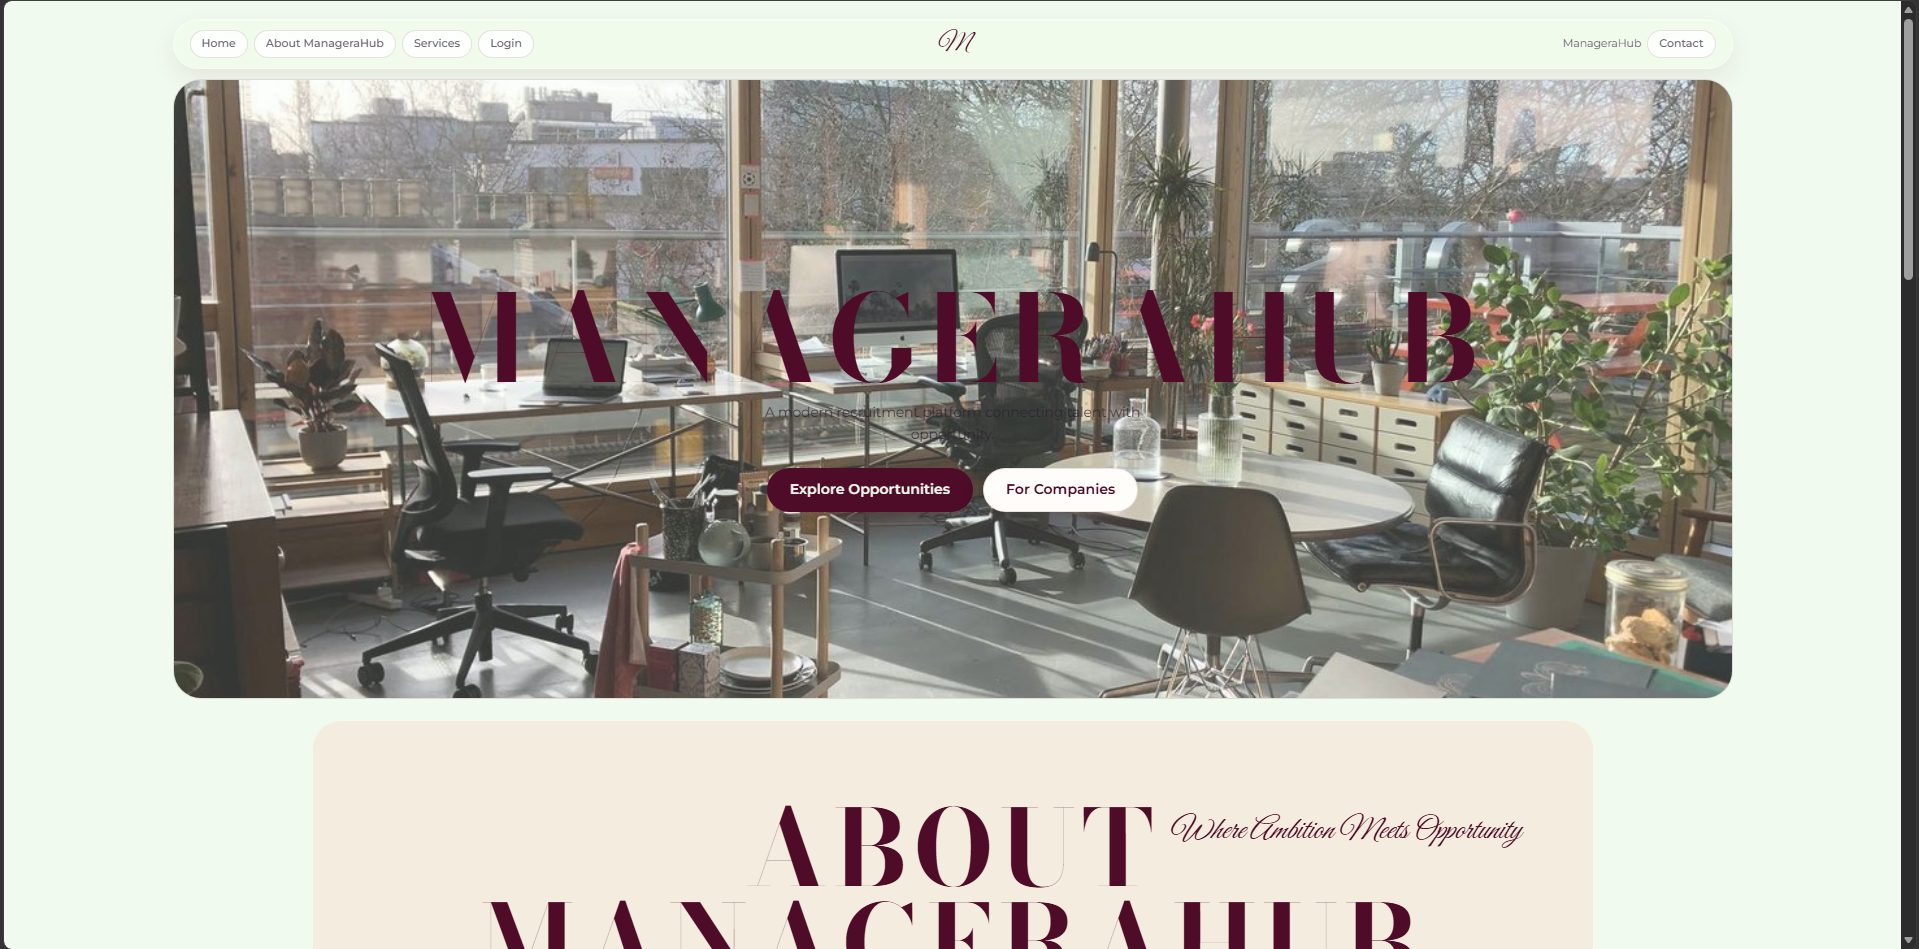
\includegraphics[width=\textwidth]{diagrams/landing.png}
    \caption{Page d'accueil de ManageraHub - Vue Desktop}
    \label{fig:landing_desktop}
\end{figure}

\begin{figure}[H]
    \centering
    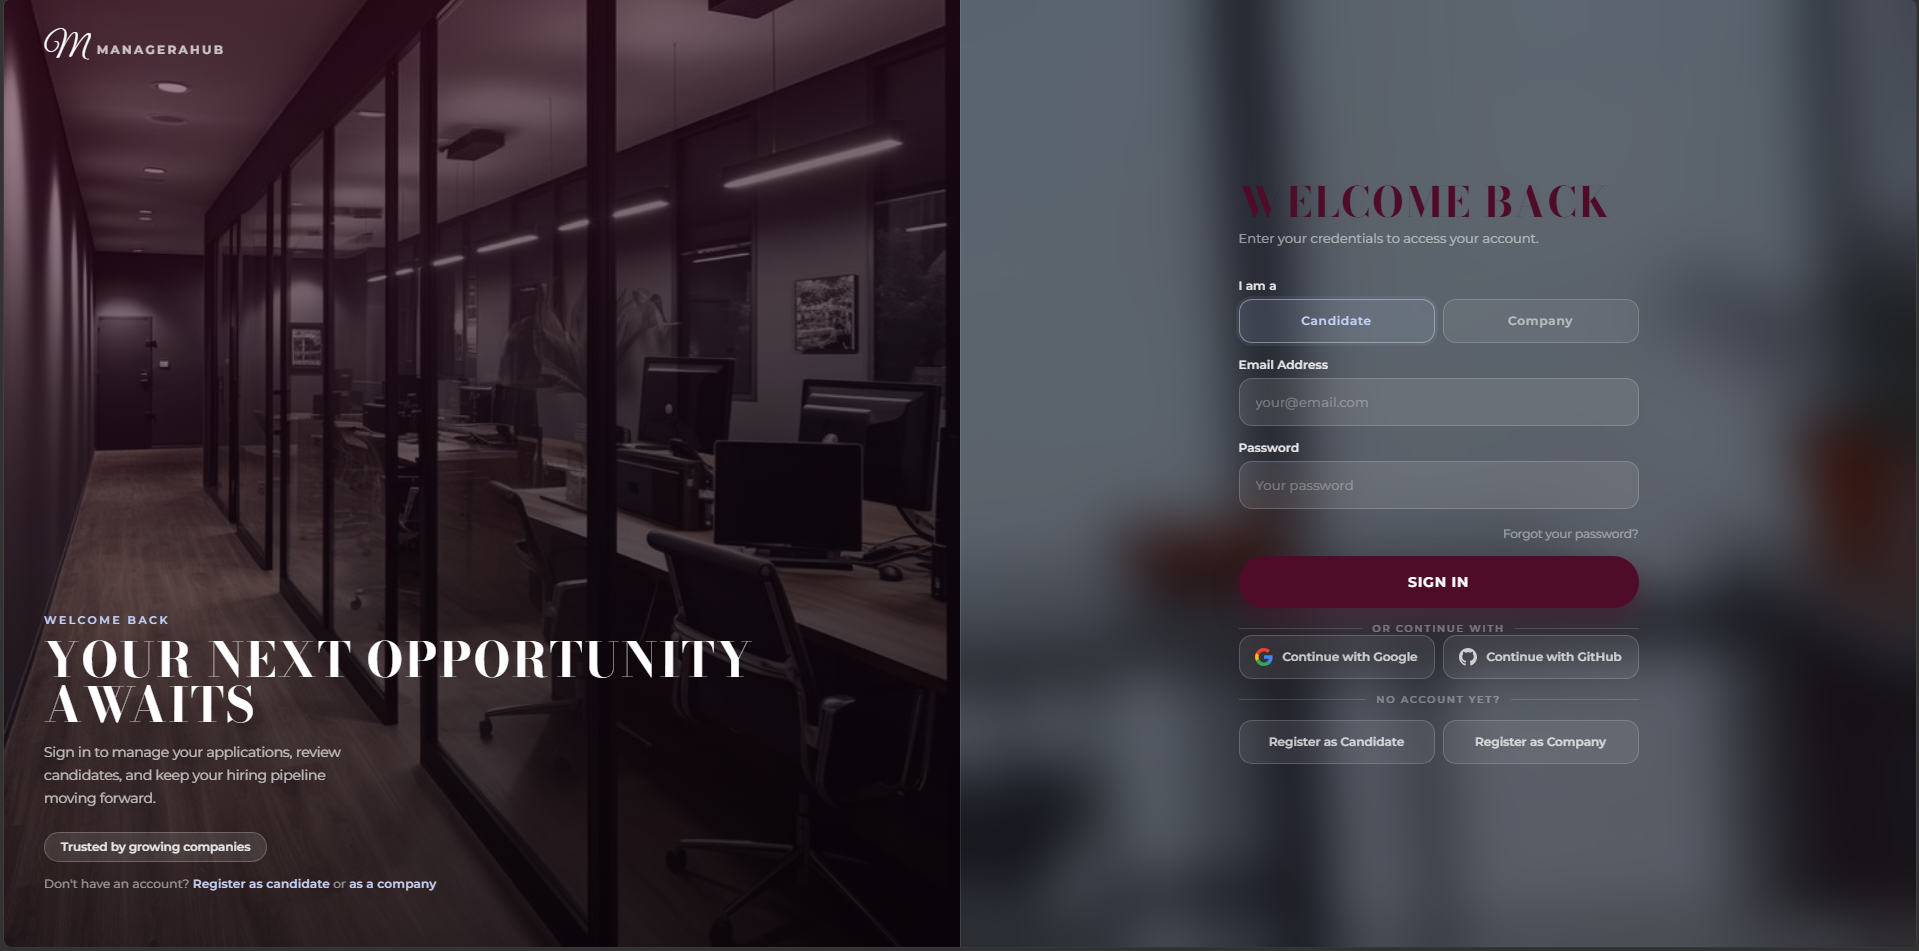
\includegraphics[width=\textwidth]{diagrams/signin.png}
    \caption{Interface de Connexion et d'Inscription de ManageraHub}
    \label{fig:signin_page}
\end{figure}

\subsection{2. Espace Candidat et Tableaux de Bord}
L'espace Candidat affiche un tableau de bord complet avec le pourcentage de complétion de son profil, sa liste de candidatures actives et leurs statuts.

De plus, nous y avons intégré un module de \textbf{suivi en temps réel des candidatures (Application Tracker)}. Ce widget de type carrousel permet au candidat de visualiser graphiquement l'évolution de ses demandes via une frise chronologique interactive (étapes : \textit{Candidature envoyée, Examen en cours, Entretien planifié, Décision finale}). Les données sont synchronisées automatiquement en tâche de fond (polling asynchrone) sans nécessiter de rafraîchir manuellement la page. Si un changement d'état est détecté, un indicateur visuel de scan radar s'active temporairement et applique un effet de surbrillance lumineuse sur la frise.

Le candidat accède également au \textbf{fil d'actualité social professionnel (Social Feed)}, optimisé pour l'interactivité grâce au défilement infini (Infinite Scroll), à l'apparition progressive par squelettes de chargement (skeletons loaders), et à l'autocomplétion dynamique lors de la recherche de membres ou de tags.

\begin{figure}[H]
    \centering
    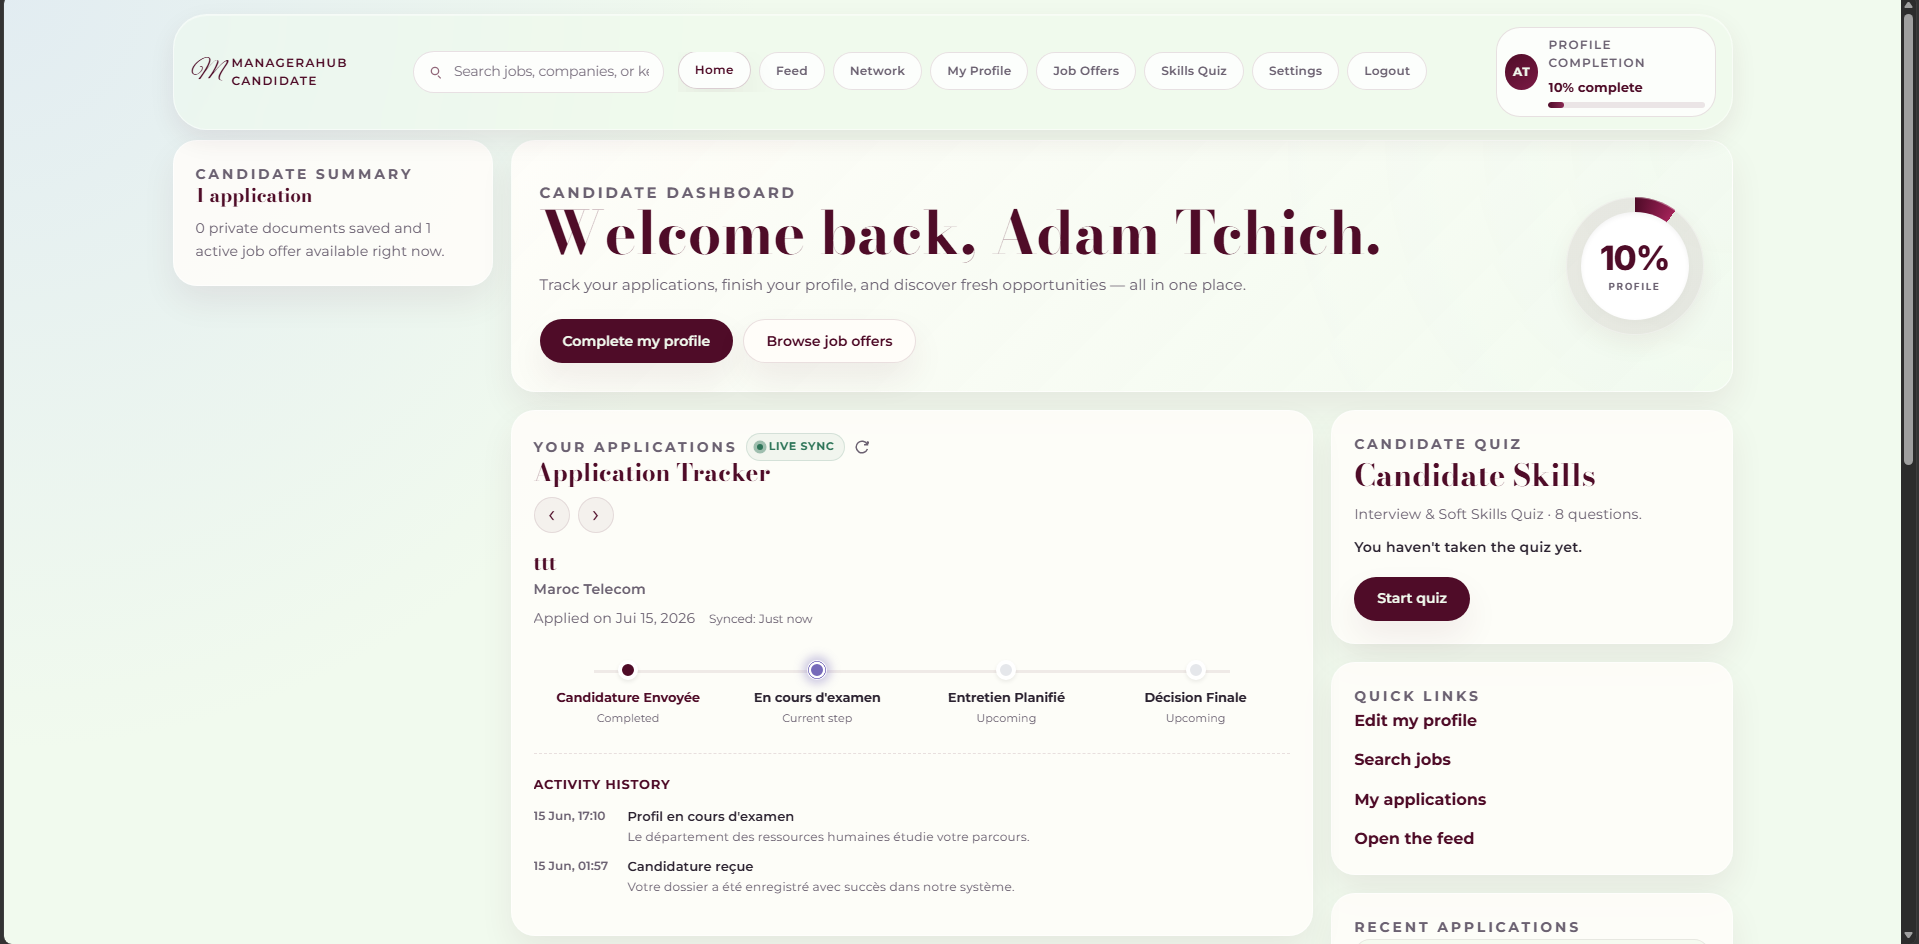
\includegraphics[width=\textwidth]{diagrams/candidate_dashboard.png}
    \caption{Tableau de bord de l'Espace Candidat avec barre de progression de profil}
    \label{fig:cand_dashboard}
\end{figure}

\begin{figure}[H]
    \centering
    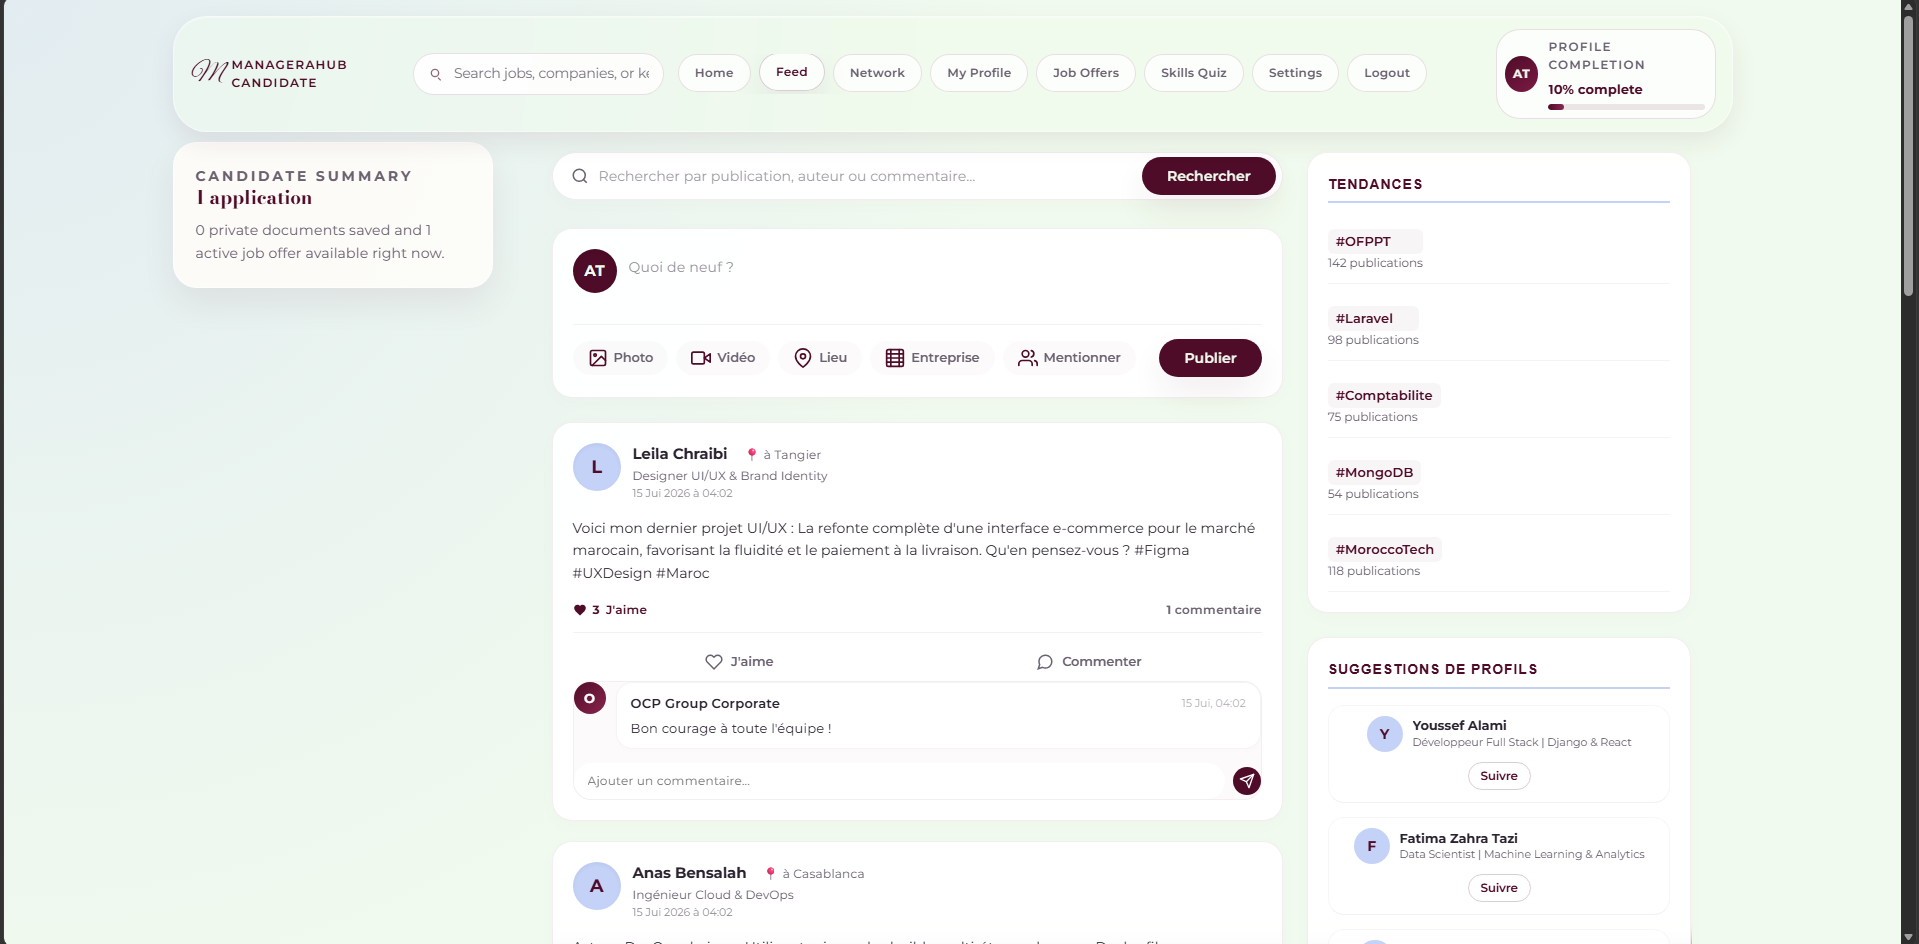
\includegraphics[width=\textwidth]{diagrams/feed.png}
    \caption{Fil d'actualités social de la plateforme avec likes et commentaires}
    \label{fig:social_feed}
\end{figure}

\subsection{3. Espace Entreprise et Gestion des Offres}
L'entreprise accède à un espace restreint permettant de gérer ses offres d'emploi actives et d'analyser les dossiers de candidature reçus.

\begin{figure}[H]
    \centering
    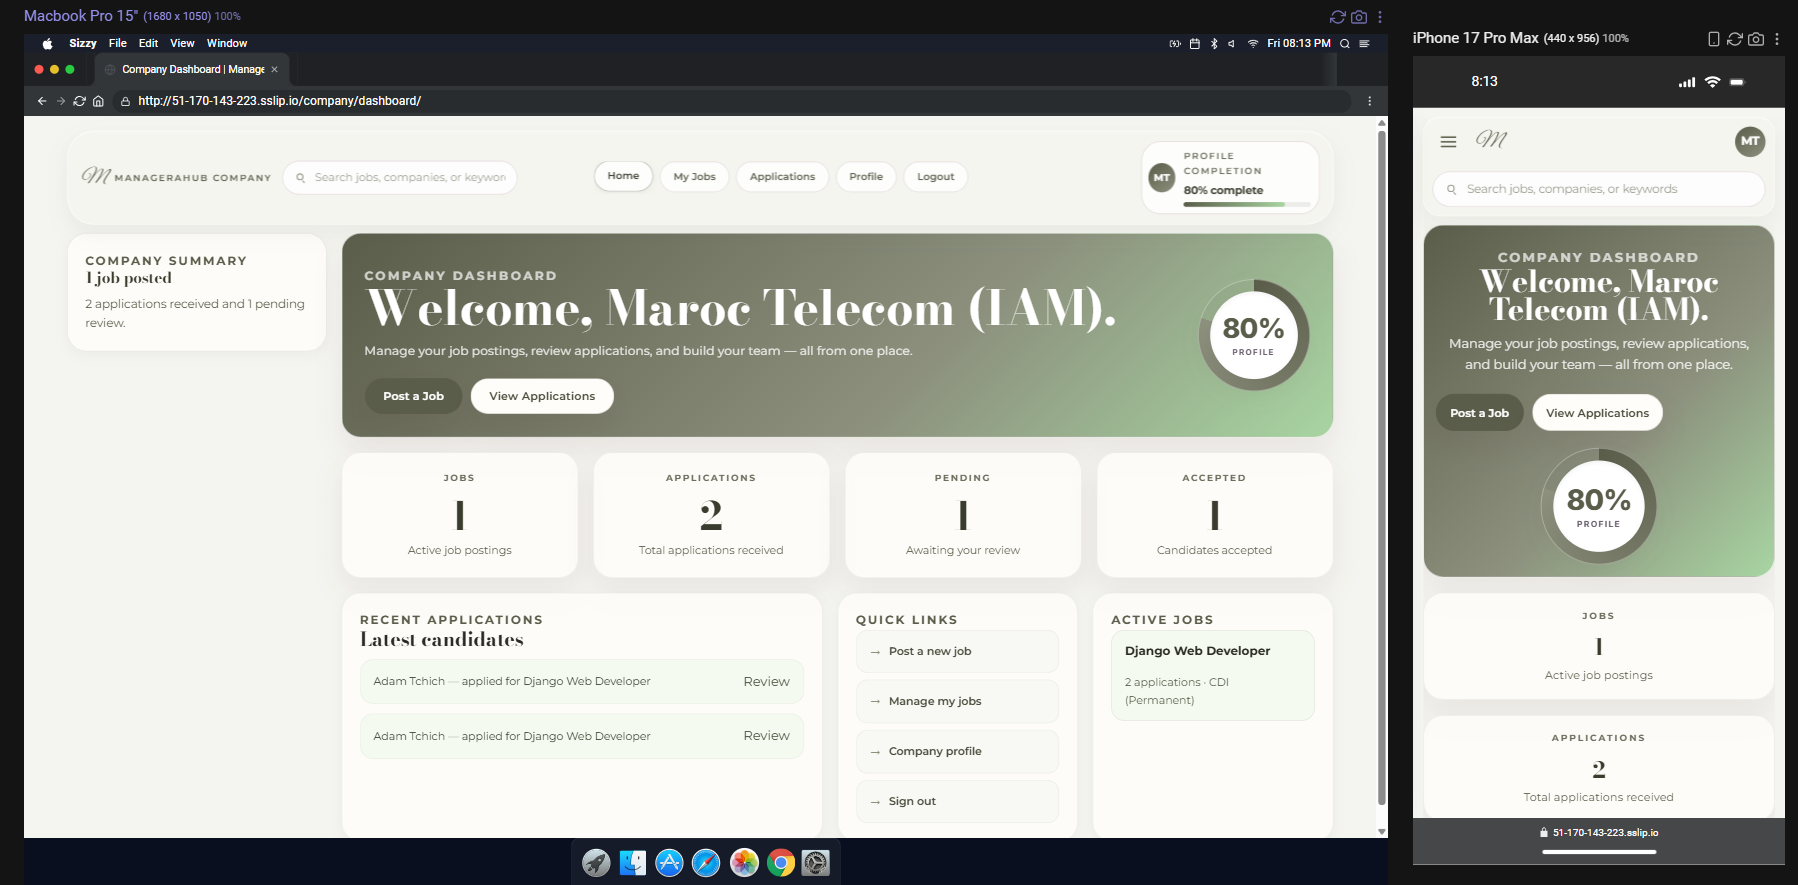
\includegraphics[width=\textwidth]{diagrams/company_dashboard.png}
    \caption{Tableau de bord de pilotage d'une Entreprise approuvée}
    \label{fig:comp_dashboard}
\end{figure}

\begin{figure}[H]
    \centering
    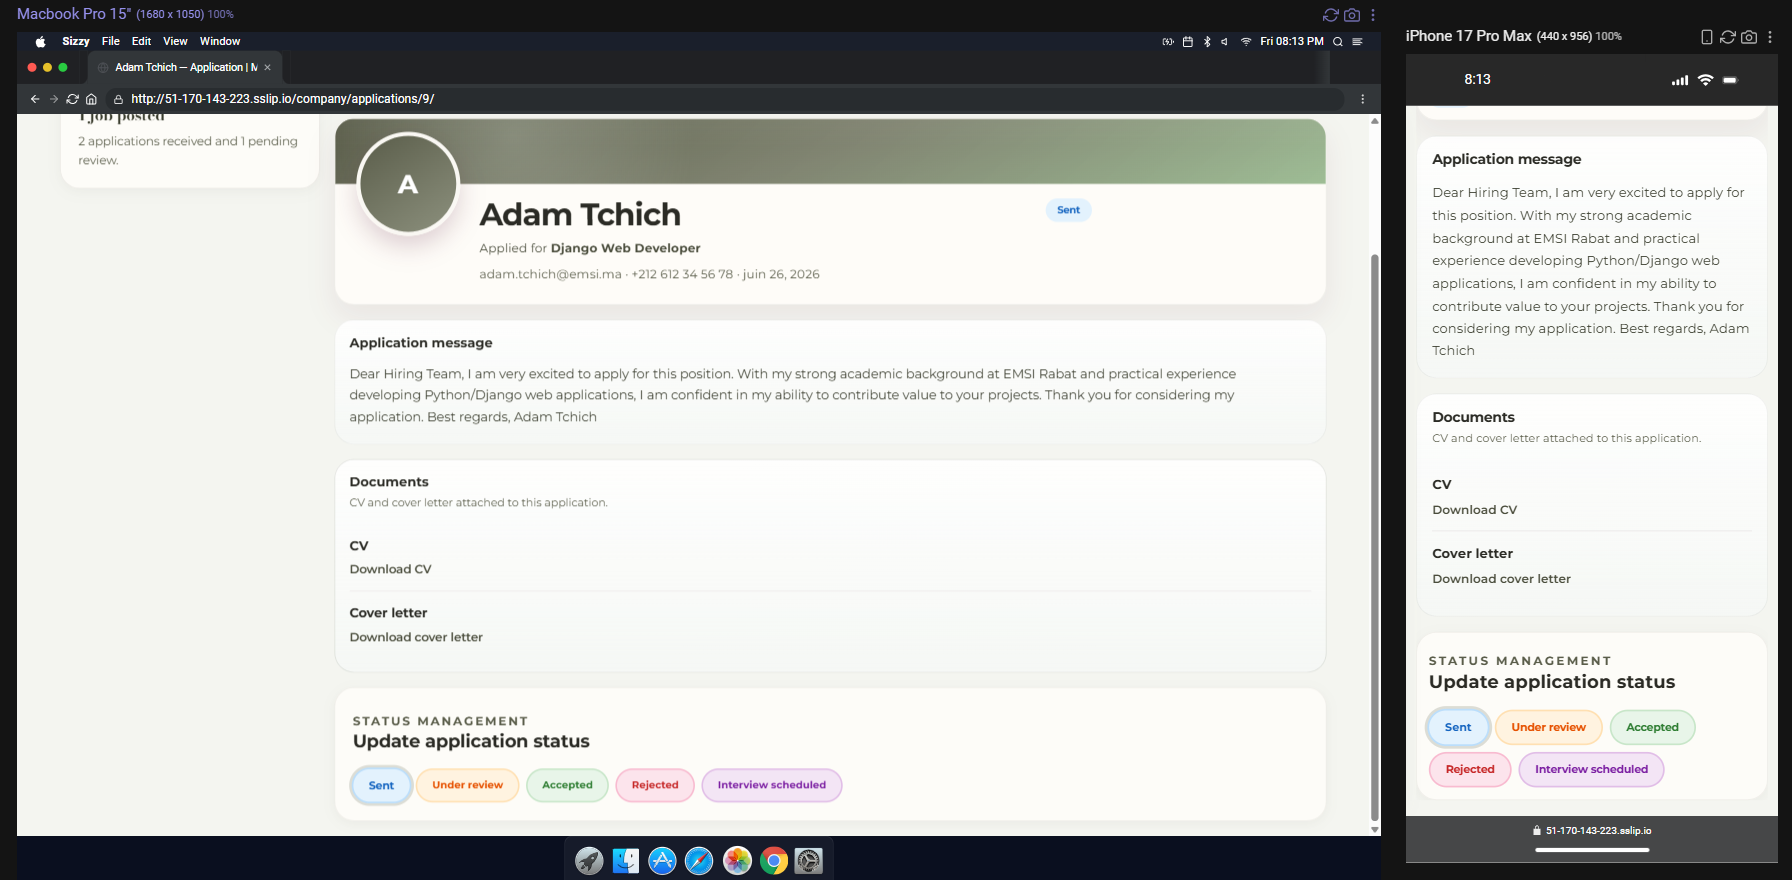
\includegraphics[width=\textwidth]{diagrams/company_application_detail.png}
    \caption{Écran d'évaluation des candidatures et de changement de statut}
    \label{fig:comp_app_detail}
\end{figure}

\subsection{4. Espace d'Administration et Modération}
Le panneau de contrôle de l'administrateur permet de vérifier les documents de légitimité de l'entreprise (ICE et RC) avant d'activer le compte.

\begin{figure}[H]
    \centering
    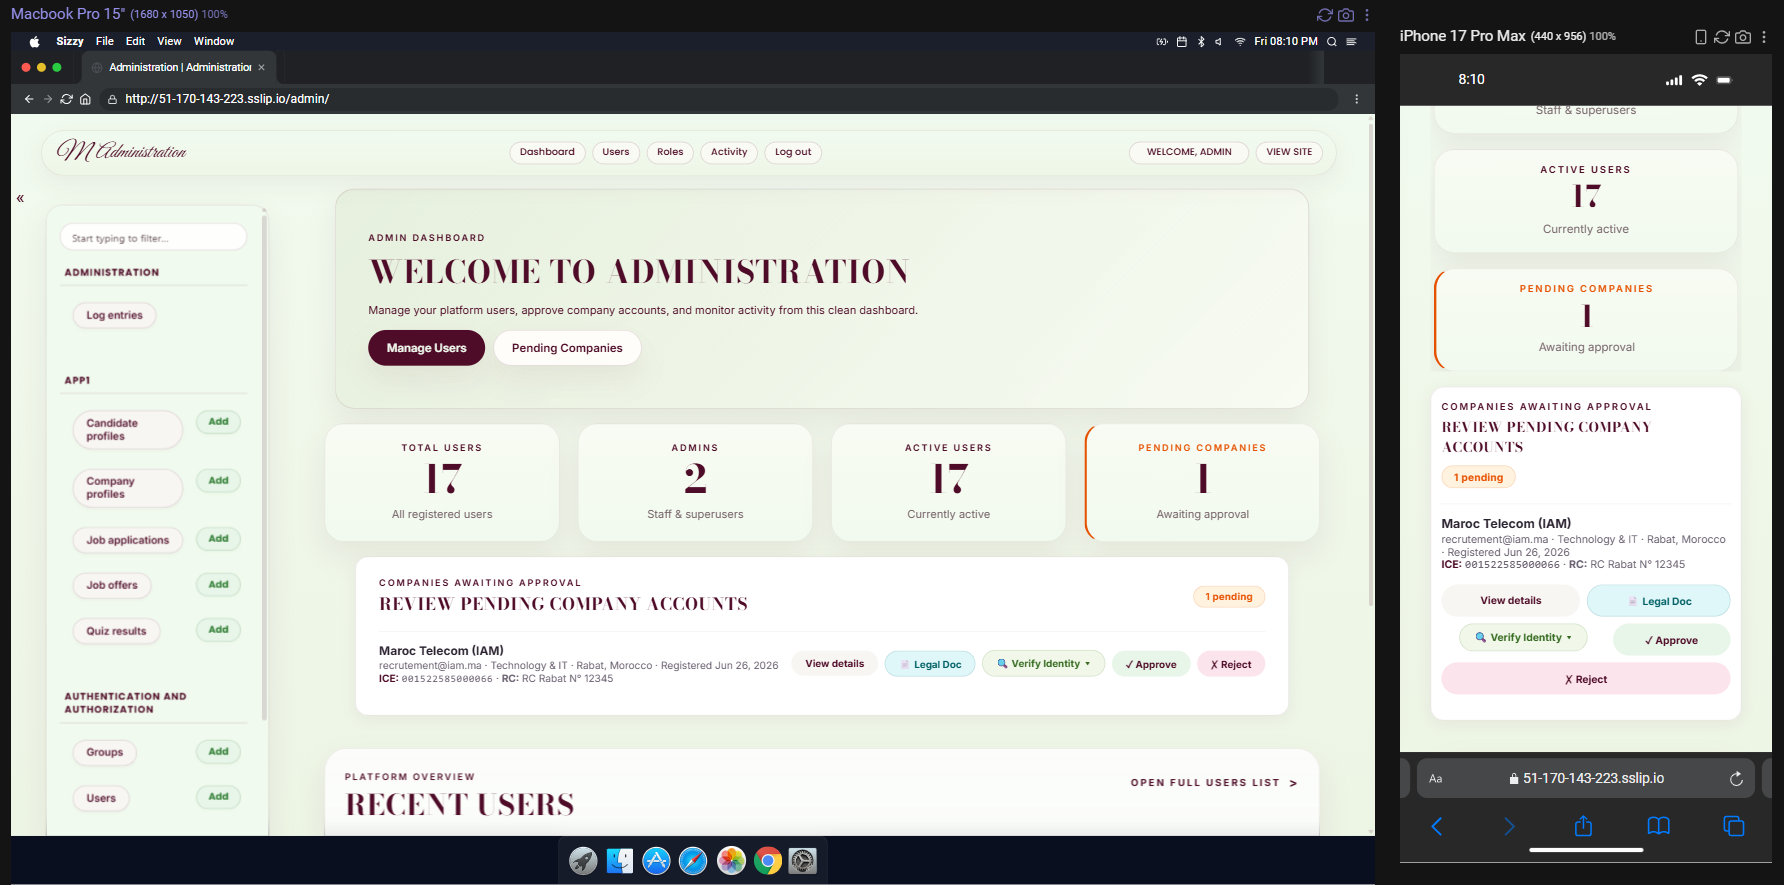
\includegraphics[width=\textwidth]{diagrams/admin_dashboard.png}
    \caption{Panneau d'administration - Validation des comptes recruteurs}
    \label{fig:admin_validation}
\end{figure}

\subsection{5. Version Mobile (Responsive Design)}
Tous les éléments graphiques se réorganisent sur les écrans mobiles et tablettes pour garantir un centrage et une lisibilité optimale.

\begin{figure}[H]
    \centering
    \includegraphics[width=\textwidth]{diagrams/mobile_responsive.png}
    \caption{Rendu de l'application ManageraHub sur écran de Smartphone}
    \label{fig:responsive_mobile}
\end{figure}

\section{Sécurité applicative mise en œuvre}
Le framework Django intègre nativement des protections contre les vulnérabilités courantes du web. Nous avons configuré et vérifié ces mécanismes :
\begin{itemize}
    \item \textbf{Protection CSRF (Cross-Site Request Forgery) :} Tous les formulaires POST génèrent un jeton unique vérifié côté serveur.
    \item \textbf{Protection XSS (Cross-Site Scripting) :} Le moteur de rendu de gabarit Django échappe automatiquement les balises HTML et JavaScript non autorisées.
    \item \textbf{Hashage des mots de passe :} Utilisation du hashage itératif PBKDF2 avec sel dynamique pour le stockage des identifiants utilisateurs.
\end{itemize}

\section{Difficultés rencontrées et solutions apportées}
Durant la phase finale d'intégration de la charte graphique et de mise en œuvre du responsive design, plusieurs défis techniques ont dû être surmontés :
\begin{enumerate}
    \item \textbf{Alignement et centrage des formulaires et des tableaux de bord :} Sur les terminaux mobiles et tablettes, certains formulaires d'authentification et de profilage apparaissaient décentrés ou présentaient des problèmes de débordement horizontal. Nous avons résolu cela en restructurant nos feuilles de style (\texttt{static/css/main.css}) pour utiliser un système de grille CSS (CSS Grid) et de boîte flexible (Flexbox) avec des marges auto-calculées, garantissant un centrage géométrique parfait de tous les boutons et entrées sur mobile.
    \item \textbf{Gestion des documents légaux :} L'ICE de l'entreprise doit obligatoirement faire 15 chiffres. Nous avons développé des validateurs personnalisés côté modèle Django (en utilisant des expressions régulières \texttt{RegexValidator}) pour bloquer l'enregistrement de valeurs invalides directement lors de la soumission du formulaire d'inscription entreprise.
    \item \textbf{Fichiers médias :} Les CV, photos de profil et lettres de motivation contiennent des informations personnelles. Pour éviter qu'ils ne soient mélangés, nous avons implémenté des fonctions de génération de chemins de stockage dynamiques et compartimentés (comme les fonctions de stockage de profil ou de candidature) qui organisent automatiquement les téléversements dans des répertoires sécurisés par identifiants d'utilisateurs et d'offres.
    \item \textbf{Mise à jour d'état en temps réel (Tracker) :} Interroger intensivement le serveur pour actualiser la timeline de candidature peut surcharger la base de données. Nous avons résolu ce problème en développant un point d'API Django dédié et optimisé qui renvoie uniquement les données JSON nécessaires, couplé à une scrutation (polling) asynchrone côté client. De plus, l'overlay de scan radar ne s'active visuellement que lorsqu'une réelle transition d'état est détectée en base de données, alliant fluidité et économie de requêtes.
    \item \textbf{Expérience fluide du fil d'actualité (Social Feed) :} Le chargement d'un grand nombre de publications avec images et vidéos ralentissait l'affichage global sur mobile. Nous avons implémenté une pagination dynamique par défilement infini (Infinite Scroll) en JavaScript. Pour combler le temps de chargement asynchrone, nous avons conçu des squelettes de chargement (skeletons loaders) animés en CSS, masquant le délai réseau et rendant l'interface fluide.
\end{enumerate}

\section{Conclusion}
La phase de réalisation s'est achevée par des phases de tests fonctionnels unitaires validant l'ensemble de la logique métier. La plateforme ManageraHub se révèle stable, sécurisée et conforme aux spécifications du cahier des charges académique.
\newpage

\chapter*{Conclusion Générale et Perspectives}
\addcontentsline{toc}{chapter}{Conclusion Générale et Perspectives}
\markboth{Conclusion Générale et Perspectives}{Conclusion Générale et Perspectives}

La conception et la réalisation de la plateforme web \textbf{ManageraHub} constituent l'aboutissement de notre Projet de Fin d'Année (PFA). Ce travail nous a permis d'apporter une réponse concrète, moderne et sécurisée aux problématiques récurrentes du marché de l'emploi en ligne au Maroc, en résolvant notamment le manque de confiance lié à la publication d'offres frauduleuses.

En introduisant une validation administrative obligatoire basée sur l'ICE et le Registre du Commerce pour les recruteurs, ManageraHub réussit à créer un espace de recrutement de confiance. En parallèle, l'intégration d'un fil d'actualités sociales professionnel a permis de transformer le profil statique classique du chercheur d'emploi en une vitrine active et interactive de ses compétences, tout en favorisant le réseautage direct.

Sur le plan académique et technique, ce projet a été particulièrement formateur. Il nous a permis d'appliquer les concepts théoriques de génie logiciel étudiés à l'EMSI, notamment à travers le processus de développement unifié \textbf{2TUP} et la modélisation UML. La mise en œuvre pratique sous le framework \textbf{Django} a renforcé nos compétences en développement backend (Python, ORM, base de données, sécurité) et frontend (ergonomie responsive et intégration dynamique).

\vspace{0.5cm}
\noindent \textbf{Perspectives d'évolution du projet :}
\begin{enumerate}
    \item \textbf{Intégration d'un algorithme de matching IA :} Développer un module d'intelligence artificielle (ex: à base de traitement du langage naturel) capable de calculer automatiquement un score d'adéquation entre le CV d'un candidat et les critères d'une offre d'emploi.
    \item \textbf{Système de notification en temps réel :} Mettre en place un serveur de WebSocket (Django Channels) pour notifier instantanément les utilisateurs des likes, commentaires, messages privés et convocations à des entretiens.
    \item \textbf{Interfaçage avec des plateformes officielles :} Automatiser la vérification de l'ICE en connectant la plateforme par API au registre public de l'OMPIC (Office Marocain de la Propriété Industrielle et Commerciale).
    \item \textbf{Espace d'entretien vidéo intégré :} Proposer un outil de visioconférence WebRTC directement accessible depuis le tableau de bord de l'entreprise pour réaliser les entretiens à distance.
\end{enumerate}

En conclusion, ManageraHub pose des bases solides pour une plateforme de recrutement innovante et sécurisée au Maroc, et constitue un jalon décisif dans notre cursus d'ingénieurs en informatique et réseaux.
\newpage

\chapter*{Références et Webographie}
\addcontentsline{toc}{chapter}{Références et Webographie}
\markboth{Références et Webographie}{Références et Webographie}

\section*{Bibliographie}
\begin{spacing}{1.3}
\begin{enumerate}[label={[\arabic*]}]
    \item \textbf{Pascal Roques}, \emph{UML 2.5 par la pratique : Cours et exercices corrigés}, Éditions Eyrolles, 2018.
    \item \textbf{Antonio Mele}, \emph{Django 4 by Example: Build powerful and reliable Python web applications}, Packt Publishing, 2022.
    \item \textbf{Vincent Drecq}, \emph{Génie logiciel et gestion de projet informatique}, Éditions Vuibert, 2015.
    \item \textbf{Marty Alchin}, \emph{Pro Django: High-performance Django web development}, Apress, 2013.
    \item \textbf{Loi 09-08 marocaine}, \emph{Relative à la protection des personnes physiques à l'égard du traitement des données à caractère personnel}.
\end{enumerate}
\end{spacing}

\vspace{1cm}

\section*{Webographie}
\begin{spacing}{1.3}
\begin{enumerate}[label={[W\arabic*]}]
    \item \textbf{Documentation officielle de Django} : \\ \url{https://docs.djangoproject.com/} (Consultée en mai 2026).
    \item \textbf{Office Marocain de la Propriété Industrielle et Commerciale (OMPIC)} : \\ \url{http://www.ompic.ma/} (Consulté en avril 2026).
    \item \textbf{Tutoriels d'optimisation de requêtes Django ORM} : \\ \url{https://realpython.com/django-orm-queries/} (Consulté en mai 2026).
    \item \textbf{W3Schools - Référence responsive CSS Grid et Flexbox} : \\ \url{https://www.w3schools.com/css/} (Consultée en avril 2026).
    \item \textbf{Mozilla Developer Network (MDN) - Web Security Guides} : \\ \url{https://developer.mozilla.org/} (Consulté en mai 2026).
    \item \textbf{Documentation de django-allauth (Authentification Sociale)} : \\ \url{https://django-allauth.readthedocs.io/} (Consultée en juin 2026).
    \item \textbf{Oracle Cloud Infrastructure (OCI) Compute Service} : \\ \url{https://docs.oracle.com/en-us/iaas/Content/Compute/} (Consulté en juin 2026).
    \item \textbf{Nginx Reverse Proxy Configuration Guide} : \\ \url{https://docs.nginx.com/nginx/admin-guide/web-server/reverse-proxy/} (Consulté en juin 2026).
    \item \textbf{Service Wildcard DNS gratuit sslip.io} : \\ \url{https://sslip.io/} (Consulté en juin 2026).
    \item \textbf{Campaign Monitor - Guide de boutons d'action hybrides (Bulletproof Buttons)} : \\ \url{https://buttons.cm/} (Consulté en juin 2026).
\end{enumerate}
\end{spacing}
\newpage

\chapter*{Annexes}
\addcontentsline{toc}{chapter}{Annexes}
\markboth{Annexes}{Annexes}

\section*{Annexe A : Guide d'installation et configuration}

Pour déployer ManageraHub en local pour le développement, veuillez suivre ces étapes :

\subsection*{1. Prérequis système}
\begin{itemize}
    \item Python 3.9 installé.
    \item Gestionnaire de paquets \texttt{pip} et utilitaire de virtualisation \texttt{venv}.
    \item Git installé pour le clonage du dépôt.
\end{itemize}

\subsection*{2. Étapes de déploiement}
\begin{lstlisting}[language=bash, caption=Commandes de configuration du projet]
# 1. Cloner le depot du projet
git clone https://github.com/TchichAdam/managerahub-django.git
cd managerahub-django

# 2. Creer et activer l'environnement virtuel
python -m venv venv
# Sur Windows :
venv\Scripts\activate
# Sur Linux/macOS :
source venv/bin/activate

# 3. Installer les dependances
pip install -r requirements.txt

# 4. Creer les fichiers de migration de base de donnees
python manage.py makemigrations app1

# 5. Appliquer les migrations
python manage.py migrate

# 6. Creer un compte administrateur principal
python manage.py createsuperuser

# 7. Lancer le serveur de developpement local
python manage.py runserver
\end{lstlisting}

Une fois le serveur démarré, l'application est accessible à l'adresse suivante dans n'importe quel navigateur web : \url{http://127.0.0.1:8000/}.

\subsection*{3. Comptes de test prédéfinis}
\begin{itemize}
    \item \textbf{Compte Administrateur :} \texttt{admin@managerahub.com} / Mot de passe : \texttt{admin123}
    \item \textbf{Candidat de test :} \texttt{candidate@}\allowbreak\texttt{test.com} / Passe : \texttt{candidate123}
    \item \textbf{Compte Entreprise de test (en attente) :} \texttt{entreprise@test.com} / Mot de passe : \texttt{entreprise123}
\end{itemize}
\textit{Note de sécurité importante : Ces comptes de test et leurs mots de passe associés sont réservés exclusivement à l'environnement de développement local (dev-only) et doivent impérativement être supprimés ou modifiés en production.}

\newpage

\section*{Annexe B : Structure des gabarits HTML (Templates)}
L'architecture de présentation (frontend) de ManageraHub est conçue selon un modèle d'héritage de templates Django, favorisant la réutilisabilité du code et le respect du principe DRY (Don't Repeat Yourself).

\subsection*{1. Fichier de base global (templates/base.html)}
Ce fichier contient la structure HTML5 globale commune, l'intégration des polices Cormorant Garamond et Inter via Google Fonts, et le point d'inclusion de la feuille de style principale.

\begin{lstlisting}[language=HTML, caption=Structure réelle du template base.html]
{% load static %}
<!DOCTYPE html>
<html lang="en">
<head>
    <meta charset="UTF-8">
    <meta name="viewport" content="width=device-width, initial-scale=1.0">
    <title>{% block title %}ManageraHub{% endblock %}</title>
    <meta name="description" content="ManageraHub is a modern recruitment platform that connects candidates, companies, and administrators in one professional experience.">
    <link rel="preconnect" href="https://fonts.googleapis.com">
    <link rel="preconnect" href="https://fonts.gstatic.com" crossorigin>
    <link href="https://fonts.googleapis.com/css2?family=Cormorant+Garamond:wght@400;500;600;700&family=Inter:wght@400;500;600;700;800&display=swap" rel="stylesheet">
    <link rel="stylesheet" href="{% static 'css/main.css' %}?v=20260615-feed-v11">
</head>
<body>
    {% block content %}{% endblock %}
    <script src="{% static 'js/main.js' %}?v=20260520-2"></script>
    {% block extra_scripts %}{% endblock %}
</body>
</html>
\end{lstlisting}

\subsection*{2. Fichier de tableau de bord Candidat (\texttt{candidate/}\allowbreak\texttt{dashboard.html})}
Ce gabarit affiche le profil du candidat, la complétion de son profil et ses candidatures récentes. Il hérite du gabarit \texttt{candidate/}\allowbreak\texttt{base.html}.

\begin{lstlisting}[language=HTML, caption=Template du Dashboard Candidat (Extrait)]
{% extends "candidate/base.html" %}

{% block title %}Candidate Dashboard | ManageraHub{% endblock %}

{% block candidate_main %}
<section class="candidate-hero-card candidate-welcome">
    <div class="candidate-welcome-text">
        <p class="candidate-card-kicker">Candidate Dashboard</p>
        <h1>Welcome back, {{ candidate_display_name }}.</h1>
        <p>Track your applications, finish your profile, and discover fresh opportunities.</p>
        <div class="candidate-hero-actions">
            <a href="{% url 'candidate_profile' %}" class="pill-button pill-button-dark">Complete my profile</a>
            <a href="{% url 'candidate_job_offers' %}" class="pill-button pill-button-light">Browse job offers</a>
        </div>
    </div>
    <div class="candidate-welcome-aside">
        <div class="candidate-progress-ring" style="--p: {{ candidate_completion_percent }};">
            <div class="candidate-progress-ring-center">
                <strong>{{ candidate_completion_percent }}%</strong>
                <span>Profile</span>
            </div>
        </div>
    </div>
</section>

<section class="candidate-dash-grid">
    <div class="candidate-dash-main">
        <article class="candidate-panel-card">
            <p class="candidate-card-kicker">Recent applications</p>
            {% if applications %}
            <div class="candidate-mini-stack">
                {% for application in applications %}
                <div class="candidate-mini-entry">
                    <strong>{{ application.job_offer.title }}</strong>
                    <span>{{ application.job_offer.company_name }} - {{ application.get_status_display }}</span>
                </div>
                {% endfor %}
            </div>
            {% else %}
            <p>You have not applied to a job yet. Start from the Job Offers page.</p>
            {% endif %}
        </article>
    </div>
</section>
{% endblock %}
\end{lstlisting}

\newpage

\section*{Annexe C : Validations de formulaires et logique de sécurité}
Pour garantir la cohérence des données, notamment pour le marché marocain, des mécanismes de validation stricts ont été mis en œuvre.

\subsection*{1. Validateur personnalisé d'ICE marocain (app1/forms.py)}
L'ICE (Identifiant Commun de l'Entreprise) doit être composé de 15 chiffres. Voici comment ce contrôle est géré dans notre formulaire de modification du profil de l'entreprise :

\begin{lstlisting}[language=Python, caption=Validation de l'ICE dans CompanyProfileForm]
from django import forms
from .models import CompanyProfile

class CompanyProfileForm(forms.ModelForm):
    class Meta:
        model = CompanyProfile
        fields = [
            "company_name",
            "industry",
            "company_size",
            "phone_number",
            "city",
            "country",
            "website",
            "description",
            "logo",
            "background_image",
            "ice",
            "rc_number",
            "legal_document",
        ]
        
    def clean_ice(self):
        ice = self.cleaned_data.get("ice")
        if ice:
            ice = ice.strip()
            if not ice.isdigit() or len(ice) != 15:
                raise forms.ValidationError("The ICE number must contain exactly 15 digits.")
        return ice
\end{lstlisting}
\newpage


\end{document}
